% Generated from Paper/manuscript; edit Markdown source.
\section{问题三：可解释融合与证据定位}
\hypertarget{q3-ux5efaux6a21ux5047ux8bbe}{%
\subsection{建模假设}\label{q3-ux5efaux6a21ux5047ux8bbe}}

假设1：题目给定的对齐位置可以作为三模态局部读出的共同索引。该索引用于模型计算；机器估计的媒体时间只用于证据回查，不假设其等于原音视特征的精确提取时间。

假设2：无有效数值的音视行不提供局部观测信息，对应项和关联交互置零。缺失状态本身不被赋予正向、负向或中性含义；是否缺失以原始观测掩码判断。

假设3：在上下文化局部编码之后，用单模态项与两两交互近似融合关系，不另设不可分解的融合残差。三方高阶作用未被显式建模，由此得到可核算性与表达能力之间的折中。

假设4：单模态回归残差的条件方差可作为该模态读出的相对可靠性线索。此假设用于构造缩放系数；是否提高泛化性能需由数据检验，方差不直接视为分类置信度或人类证据可信程度。

\hypertarget{q3-ux6570ux636eux89c2ux5bdfux4e0eux9884ux5904ux7406}{%
\subsection{数据观察与预处理}\label{q3-ux6570ux636eux89c2ux5bdfux4e0eux9884ux5904ux7406}}

使用附件二训练与验证划分建立模型，附件四20条无标签样本用于专项预测与解释。

每条样本最多50个对齐位置，给定文本特征768维、语音特征74维、视觉特征35维，另有BERT词元编号、注意力掩码及类型编号。本模型选择text\_bert输入预训练BERT\cite{q2-ref1}，不把text与text\_bert视为两个模态。剔除特殊词元和填充位置后保留原序列位置source\_index，文本隐状态经LayerNorm后回填到局部窗口。

语音、视觉全零行按无有效数值观测处理。对模态m的第d维，仅在训练集有效观测上计算均值μₘd和总体标准差sₘd，并标准化为(xₘⱼd−μₘd)/sₘd；标准差小于10⁻⁶时置为1。缺失行保持为零且保留掩码，验证、测试和附件四复用训练统计，避免把待评价集合的信息用于归一化参数估计。

模型评估基于既有探索实验：历史研究中曾多次查看附件二测试表现，最终方案同时考虑已有性能与解释要求。因而本文报告的是单种子探索性比较，不能作为完全独立、确认性的模型优越性结论；附件四在正式展示中只报告模型输出。

\hypertarget{q3-ux6a21ux578bux5efaux7acb}{%
\subsection{模型建立}\label{q3-ux6a21ux578bux5efaux7acb}}

\hypertarget{q3-ux4e0aux4e0bux6587ux5316ux5c40ux90e8ux8bc1ux636eux4e0eux6210ux5bf9ux4ea4ux4e92}{%
\subsubsection{上下文化局部证据与成对交互}\label{q3-ux4e0aux4e0bux6587ux5316ux5c40ux90e8ux8bc1ux636eux4e0eux6210ux5bf9ux4ea4ux4e92}}

借鉴神经可加模型\cite{q3-ref2}与成对交互建模\cite{q3-ref3}，采用``局部非线性编码---显式加性读出''的结构。BERT提供语言上下文，局部编码保留证据位置，成对分支表达同位置的跨模态共同作用。可靠性缩放在样本层调整这些读出项，不额外设置无法核算的融合残差。预测及解释共享同一次前向中的实际数值。

\begin{figure}
\centering
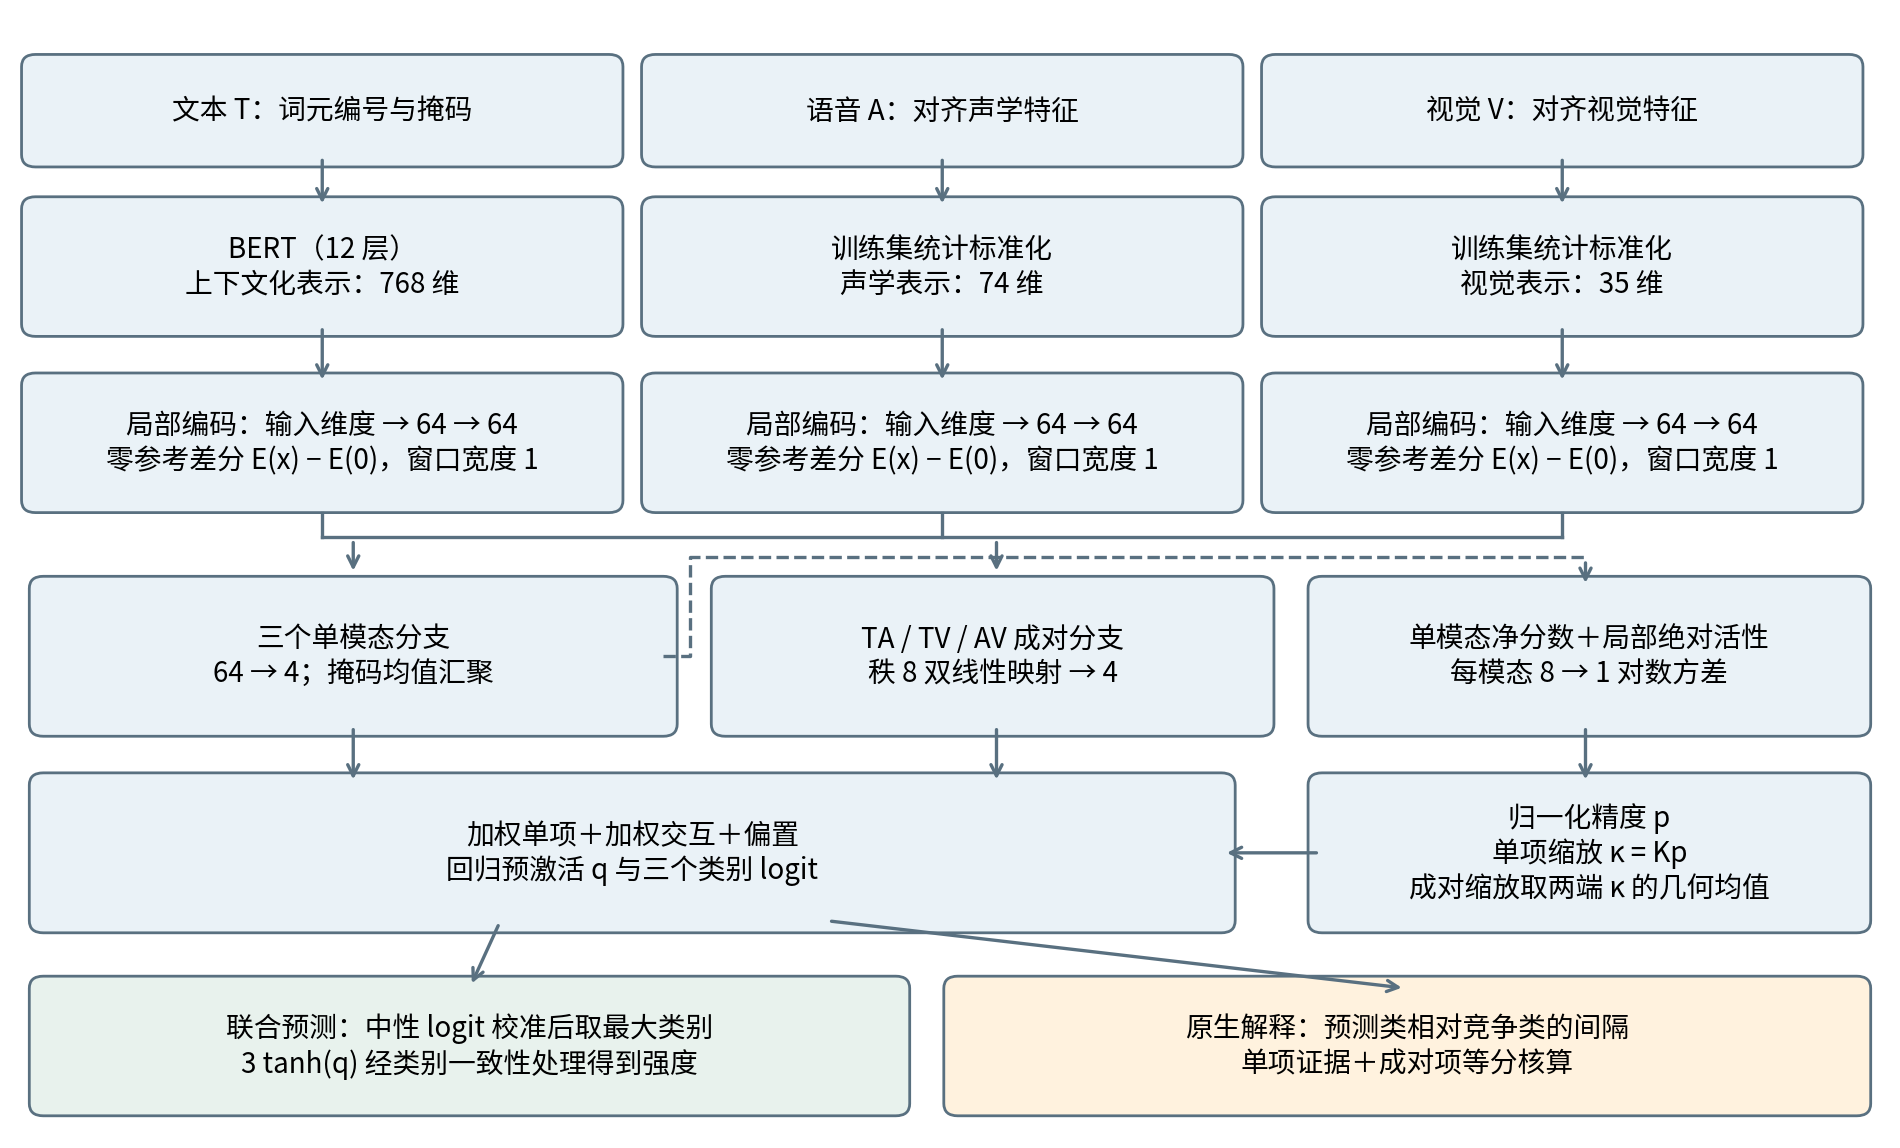
\includegraphics{../问题3/paper/figures/01_network.png}
\caption{不确定性融合网络。T/A/V为文本/语音/视觉；每个分支的4维输出对应q及负向、中性、正向logit。\label{q3-fig2}}
\end{figure}

记m∈\{T,A,V\}，j为有效内容窗口。窗口宽度为1；每模态局部编码器由逐行线性映射与GELU、窗口拼接线性映射与GELU构成，投影维度与局部隐层均为64。文本BERT隐状态先作LayerNorm，再按source\_index回填局部位置。用相同观测结构下的零输入编码作为参考，得到下式。参考为特征坐标基准，不代表真实中性情绪。

\begin{equation}
\begin{gathered}d_{mj}=E_m(x_{mj},o_{mj})-E_m(0,o_{mj})\end{gathered}\label{q3-eq1}
\end{equation}

单模态读出为无偏置64→4线性映射。均值汇聚权重ωₘⱼ正比于该窗口内有效观测数；成对权重ωₘₙⱼ以两端权重几何均值构造，限制在共同有效窗口，再按样本归一化。TA、TV、AV各使用独立的秩8双线性投影，分别输出4维交互。

\begin{equation}
\begin{gathered}a_{mj}=\omega_{mj}W_md_{mj},\quad i_{mnj}=\omega_{mnj}V_{mn}[(P_{mn}d_{mj})\odot(Q_{mn}d_{nj})]\end{gathered}\label{q3-eq2}
\end{equation}

P、Q、V均不含偏置；某一模态没有有效观测时，该单项与关联交互严格为零。BERT使单个文本读出含有全句上下文，因此局部值解释为该位置的上下文化读出。成对模块连接对齐位置，文本上下文来自BERT，模型不另设音视跨位置注意力或三方高阶交互。

\hypertarget{q3-ux7531ux6b8bux5deeux65b9ux5deeux9a71ux52a8ux7684ux53efux9760ux6027ux878dux5408}{%
\subsubsection{由残差方差驱动的可靠性融合}\label{q3-ux7531ux6b8bux5deeux65b9ux5deeux9a71ux52a8ux7684ux53efux9760ux6027ux878dux5408}}

首先从未进行精度缩放的单项计算每模态四维净分数uₘ=β+Σⱼaₘⱼ，同时统计各输出维度局部读出的绝对活性Σⱼ\textbar aₘⱼ\textbar。拼接后得到8维输入，通过每模态一个8→1线性层预测有界对数方差。训练时活性来自模态丢弃后的单项，单模态监督仍使用丢弃前的实际单项。

\begin{equation}
\begin{gathered}v_m=-1+4\tanh(w_m^{\mathsf T}[u_m;\sum_j\mathrm{abs}(a_{mj})]+b_m),\quad \sigma_m^2=\exp(v_m)\end{gathered}\label{q3-eq3}
\end{equation}

\begin{equation}
\begin{gathered}p_m=\frac{\mathbf1_m\exp(-v_m)}{\sum_n\mathbf1_n\exp(-v_n)},\quad \kappa_m=Kp_m,\quad K=\sum_m\mathbf1_m\end{gathered}\label{q3-eq4}
\end{equation}

1ₘ表示当前保留且可观测的模态。单项按κₘ缩放，成对项按√(κₘκₙ)缩放。精度相同时κₘ=1，恢复基础加性读出；方差被限制在exp(−5)至exp(3)之间。方差监督针对单模态回归残差，它既不是分类概率校准，也不是融合后预测区间。归一化精度pₘ是可靠性系数，其定义与模态净贡献占比不同。

\begin{equation}
\begin{gathered}s=\beta+\sum_{m,j}\kappa_m a_{mj}+\sum_{(m,n)\in\mathcal P,j}\sqrt{\kappa_m\kappa_n}\,i_{mnj} \\ q=s_0,\quad \ell=(s_1,s_2,s_3)\end{gathered}\label{q3-eq5}
\end{equation}

P=\{(T,A),(T,V),(A,V)\}为无序模态对的集合，每个成对项只计入一次。

\hypertarget{q3-ux8054ux5408ux8f93ux51faux4e0eux6a21ux6001ux8d21ux732eux5b9aux4e49}{%
\subsubsection{联合输出与模态贡献定义}\label{q3-ux8054ux5408ux8f93ux51faux4e0eux6a21ux6001ux8d21ux732eux5b9aux4e49}}

回归原始输出\(r=3\tanh(q)\)。冻结分类策略为中性logit加−0.4后取最大值：\(\ell^{\prime}=\ell+(0,-0.4,0)\)，\(\hat c=\arg\max_c\ell^{\prime}_c\)。最终强度按类别保持符号一致：负向min(r,−10⁻⁶)，中性0，正向max(r,10⁻⁶)。所有主表MAE均评价该最终强度，同时另存raw\_intensity。分类和回归共享全部编码及交互参数，输出层有各任务对应的行，联合训练；主模型未启用有序分类头，但保留强度的有序辅助损失。

对每条样本，以预测类别ĉ与最强竞争类别c₂的校准logit差M=ℓ′ĉ−ℓ′c₂为分类解释目标。将所有4维读出投影到这一类别差后，记单模态总项Aₘ、交互总项Iₘₙ。每个成对交互的一半分配给相关两端，得到模态净分数与位置净分数：

\begin{equation}
\begin{gathered}\Phi_m=A_m+\frac12\sum_{n\ne m}I_{mn},\quad\psi_{mj}=\tilde{a}_{mj}+\frac12\sum_{n\ne m}\tilde{i}_{mnj} \\ M=\beta_M+\sum_m\Phi_m\end{gathered}\label{q3-eq6}
\end{equation}

\begin{equation}
\begin{gathered}\rho_m=\frac{\mathrm{abs}(\Phi_m)}{\sum_n\mathrm{abs}(\Phi_n)},\quad m_{\mathrm{ref}}=\mathrm{argmax}_m\,\mathrm{abs}(\Phi_m)\end{gathered}\label{q3-eq7}
\end{equation}

ã和ĩ表示已缩放、已投影到解释目标的读出。βM包括两个对应输出偏置之差，以及中性−0.4校准项对该类别差的影响。解释卡同时保留符号：正值支持预测类别相对于竞争类别，负值反对该判断。ρ采用模态净值的绝对值归一化，偏置βM单列；它不同于把所有局部绝对值先相加得到的活性比例。若分母近零则标为未定义，主要模态不能强制指定。回归解释以q为目标同样核算，相应比例描述q的加性分解。动态可靠性与BERT上下文均随输入变化，因此当前分数项删除不等于重新运行被修改输入后的输出变化。

\hypertarget{q3-ux6a21ux578bux6c42ux89e3ux4e0eux8badux7ec3ux65b9ux6848}{%
\subsection{模型求解与训练方案}\label{q3-ux6a21ux578bux6c42ux89e3ux4e0eux8badux7ec3ux65b9ux6848}}

\hypertarget{q3-ux591aux4efbux52a1ux76eeux6807ux51fdux6570}{%
\subsubsection{多任务目标函数}\label{q3-ux591aux4efbux52a1ux76eeux6807ux51fdux6570}}

\begin{equation}
\begin{gathered}L=L_{\mathrm{Huber}}(r,y)+0.5L_{\mathrm{CE}}(\ell,c)+0.1L_{\mathrm{ord}}+0.001L_{\mathrm{pair}} \\ \quad+0.1L_{\mathrm{uni}}+0.1L_{\mathrm{neutral}}+0.1L_{\mathrm{polarity}}+0.1L_{\mathrm{NLL}}\end{gathered}\label{q3-eq8}
\end{equation}

Huber阈值δ=1。Lpair为每样本所有已缩放成对项回归分量的绝对值之和，再在批内平均。Luni在实际可观测模态上平均Huber单模态回归损失与0.5倍单模态交叉熵；它使用uₘ的回归、分类分量。Lneutral使用中性logit减去正负logsumexp作为二分类log-odds；Lpolarity仅在非中性样本上对正负logit差进行二元交叉熵。Lord用固定带宽0.3、温度0.2构造两个累计logit：((r+0.3)/0.2, (r−0.3)/0.2)，分别以1{[}c\textgreater0{]}和1{[}c\textgreater1{]}为目标计算二元交叉熵并平均；该项不是启用独立的可学习有序头。

\begin{equation}
\begin{gathered}e_{im}=3\tanh(u_{im0})-y_i \\ L_{\mathrm{NLL}}=\frac{1}{2N_{\mathcal O}}\sum_{(i,m)\in\mathcal O}(\exp(-v_{im})e_{im}^2+v_{im})\end{gathered}\label{q3-eq9}
\end{equation}

式\eqref{q3-eq9}在批内所有实际可观测的``样本---模态''对上取平均，记这些索引对的集合为O、数量为N\_O；abs表示绝对值。i为样本索引，uᵢₘ,₀为对应单模态读出的回归分量。模态丢弃不改变此项的实际观测监督范围。

异方差回归的NLL建模\cite{q3-ref4}用于单模态残差方差，使可靠性模块获得可监督训练信号。该损失不是三模态贡献的监督真值，预测方差的绝对大小不能直接等同于人类对证据可靠性的判断。整个模型用AdamW更新，BERT编码层和其他层使用固定分组学习率，学习率固定。

\hypertarget{q3-ux6c42ux89e3ux6d41ux7a0bux4e0eux5173ux952eux53c2ux6570}{%
\subsubsection{求解流程与关键参数}\label{q3-ux6c42ux89e3ux6d41ux7a0bux4e0eux5173ux952eux53c2ux6570}}

训练环境为Python 3.11.15、PyTorch 2.5.1+cu124、NumPy 2.4.6和RTX 3090 Ti。推理加载固定检查点与训练统计，使用与训练相同的对齐输入。

求解分为五步：①在附件二训练集估计有效观测的标准化统计量；②载入公开预训练BERT，初始化局部编码、成对读出与方差模块；③按批次执行模态丢弃、联合前向与目标函数求导，使用AdamW更新参数；④每轮在验证集比较分类策略，保存三个选优目标对应的检查点；⑤选择固定检查点与决策策略，在测试集计算评价指标，在附件四输出预测及解释。附件四不参与上述训练和验证策略搜索。

\begin{PaperTable}{2}

\begin{longtable}[]{@{}ll@{}}
\caption{主模型训练与推理参数\label{q3-tab3}}\tabularnewline
\toprule
\begin{minipage}[b]{0.42\columnwidth}\raggedright
参数\strut
\end{minipage} & \begin{minipage}[b]{0.52\columnwidth}\raggedright
冻结主模型设置\strut
\end{minipage}\tabularnewline
\midrule
\endfirsthead
\caption[]{主模型训练与推理参数（续）}\tabularnewline
\toprule
\begin{minipage}[b]{0.42\columnwidth}\raggedright
参数\strut
\end{minipage} & \begin{minipage}[b]{0.52\columnwidth}\raggedright
冻结主模型设置\strut
\end{minipage}\tabularnewline
\midrule
\endhead
\begin{minipage}[t]{0.42\columnwidth}\raggedright
随机种子 / 批大小\strut
\end{minipage} & \begin{minipage}[t]{0.52\columnwidth}\raggedright
17 / 32\strut
\end{minipage}\tabularnewline
\begin{minipage}[t]{0.42\columnwidth}\raggedright
BERT / 其他层学习率\strut
\end{minipage} & \begin{minipage}[t]{0.52\columnwidth}\raggedright
2×10⁻⁵ / 3×10⁻⁴，固定\strut
\end{minipage}\tabularnewline
\begin{minipage}[t]{0.42\columnwidth}\raggedright
AdamW权重衰减 / 梯度裁剪\strut
\end{minipage} & \begin{minipage}[t]{0.52\columnwidth}\raggedright
0.01（二维以上参数）/ 1.0\strut
\end{minipage}\tabularnewline
\begin{minipage}[t]{0.42\columnwidth}\raggedright
窗口 / 行投影 / 局部维度 / 交互秩\strut
\end{minipage} & \begin{minipage}[t]{0.52\columnwidth}\raggedright
1 / 64 / 64 / 8\strut
\end{minipage}\tabularnewline
\begin{minipage}[t]{0.42\columnwidth}\raggedright
局部dropout / 模态丢弃率\strut
\end{minipage} & \begin{minipage}[t]{0.52\columnwidth}\raggedright
0.2 / 0.1\strut
\end{minipage}\tabularnewline
\begin{minipage}[t]{0.42\columnwidth}\raggedright
最大轮次 / 早停耐心值\strut
\end{minipage} & \begin{minipage}[t]{0.52\columnwidth}\raggedright
20 / 连续4轮三个选优目标均无刷新\strut
\end{minipage}\tabularnewline
\begin{minipage}[t]{0.42\columnwidth}\raggedright
实际轮数 / 采用检查点\strut
\end{minipage} & \begin{minipage}[t]{0.52\columnwidth}\raggedright
9 / 第5轮\strut
\end{minipage}\tabularnewline
\begin{minipage}[t]{0.42\columnwidth}\raggedright
可训练BERT层 / AMP\strut
\end{minipage} & \begin{minipage}[t]{0.52\columnwidth}\raggedright
12层，embedding和pooler冻结 / 关闭\strut
\end{minipage}\tabularnewline
\begin{minipage}[t]{0.42\columnwidth}\raggedright
总参数 / 可训练参数\strut
\end{minipage} & \begin{minipage}[t]{0.52\columnwidth}\raggedright
109,555,007 / 85,127,231\strut
\end{minipage}\tabularnewline
\begin{minipage}[t]{0.42\columnwidth}\raggedright
分类最终策略\strut
\end{minipage} & \begin{minipage}[t]{0.52\columnwidth}\raggedright
中性logit偏置−0.4；最大logit类别\strut
\end{minipage}\tabularnewline
\bottomrule
\end{longtable}

\end{PaperTable}

每轮仅在验证集搜索策略：441组回归中性阈值和31个中性logit偏置，共472个候选；分别按Macro-F1、Accuracy及最终强度MAE维护独立最佳检查点。任一目标排序刷新即重置早停计数，不是只监测训练损失。本文主表统一取验证Macro-F1策略，各指标使用相同检查点和策略。第5轮之后训练损失继续降低但验证原始MAE未刷新，支持保留早停；增加训练上限不自动增加有效训练轮数。

\begin{figure}
\centering
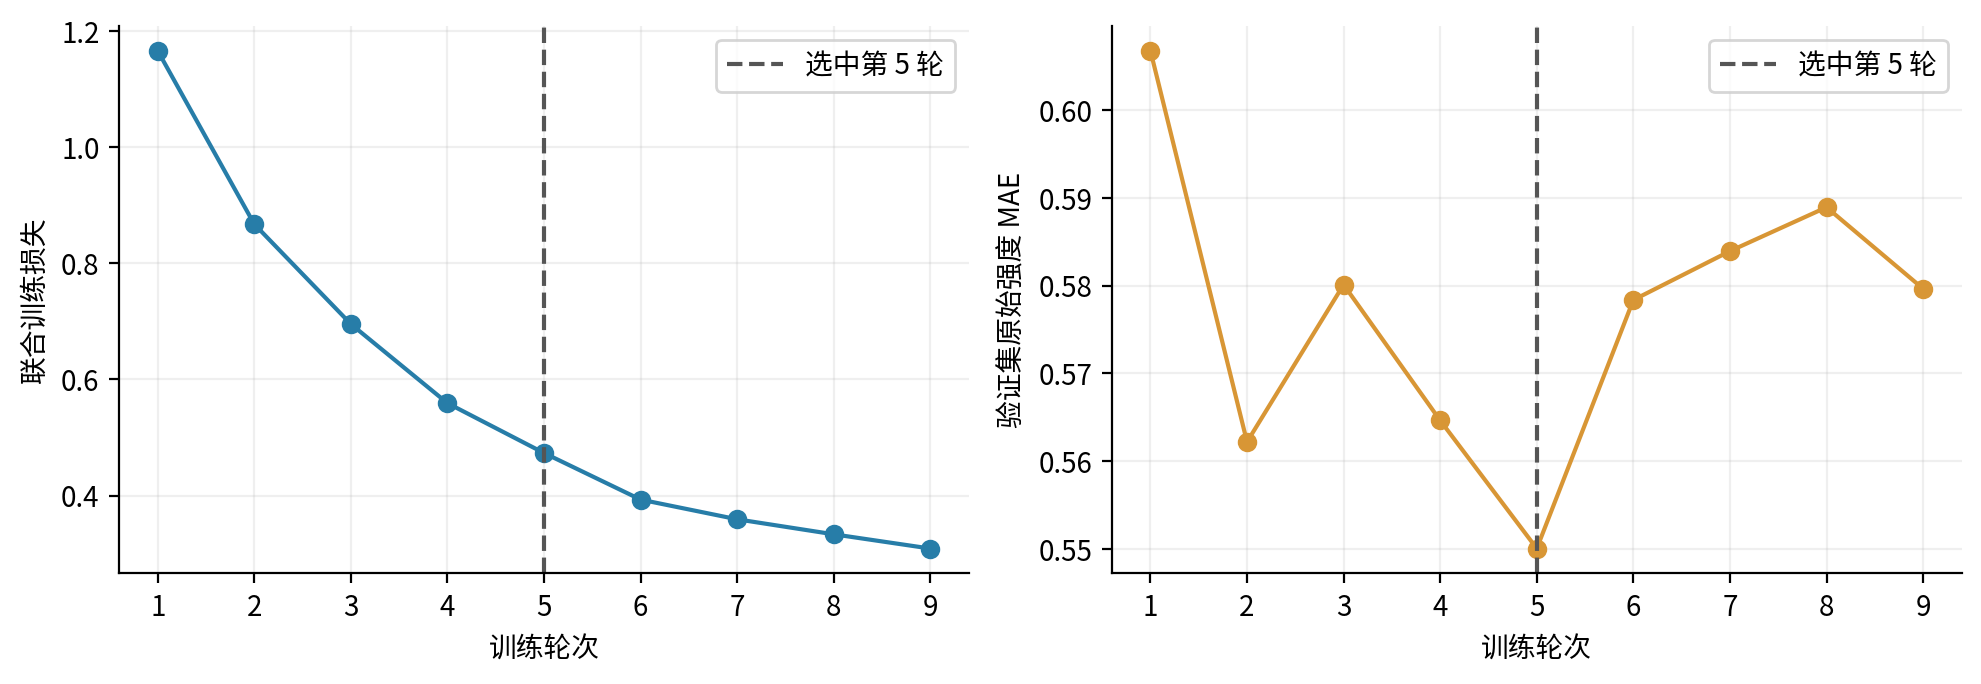
\includegraphics{../问题3/paper/figures/02_training.png}
\caption{主模型训练曲线。虚线为第5轮，实际第9轮停止。右图为原始强度MAE，区别于主表最终强度MAE。\label{q3-fig3}}
\end{figure}

\hypertarget{q3-ux8bc4ux4ef7ux6307ux6807ux4e0eux5bf9ux6bd4ux8bbeux7f6e}{%
\subsubsection{评价指标与对比设置}\label{q3-ux8bc4ux4ef7ux6307ux6807ux4e0eux5bf9ux6bd4ux8bbeux7f6e}}

附件二验证集的正向样本占46.43\%，负向和中性分别占28.30\%和25.27\%，类别分布不均衡。因此同时采用准确率、Macro-F1和中性F1评价分类，采用平均绝对误差MAE与Pearson相关系数评价强度。所有回归指标均以类别一致性处理后的最终强度计算。

各指标采用共用评价约定，三分类按负向、中性、正向计算，回归评价最终强度。

选择两个具有已训练检查点的开源适配基线。SELF-MM\cite{q3-ref5}采用BERT文本编码、音视LSTM、融合及单模态读出和中心驱动动态伪标签；本实现增加比赛三分类读出、有效观测打包与数值稳定处理。TETFN\cite{q3-ref6}直接使用MMSA工具库\cite{q3-ref7}固定版本的网络源码，恢复对齐音视位置，增加比赛分类头及有界回归输出，并使用本地联合训练目标。二者均为比赛数据适配实验，不是原论文数据规模、训练目标和配置下的严格复现。

所有方法仅以3395条训练样本学习，在同一728条验证集上选轮次和策略；本表统一使用各自验证Macro-F1版本。主模型最终按分类logit决策，而两基线的验证最优策略为回归阈值决策，策略差异一并列出，避免把结果误认为统一最后一层阈值的比较。

\hypertarget{q3-ux57faux7840ux6027ux80fdux4e0eux53efux89c6ux5316ux5206ux6790}{%
\subsubsection{基础性能与可视化分析}\label{q3-ux57faux7840ux6027ux80fdux4e0eux53efux89c6ux5316ux5206ux6790}}

\begin{PaperTable}{6}

\begin{longtable}[]{@{}llllll@{}}
\caption{验证集（728条）模型性能比较\label{q3-tab4}}\tabularnewline
\toprule
\begin{minipage}[b]{0.22\columnwidth}\raggedright
模型\strut
\end{minipage} & \begin{minipage}[b]{0.12\columnwidth}\raggedright
Acc(\%)\strut
\end{minipage} & \begin{minipage}[b]{0.12\columnwidth}\raggedright
Macro-F1\strut
\end{minipage} & \begin{minipage}[b]{0.12\columnwidth}\raggedright
MAE\strut
\end{minipage} & \begin{minipage}[b]{0.12\columnwidth}\raggedright
Pearson\strut
\end{minipage} & \begin{minipage}[b]{0.12\columnwidth}\raggedright
中性F1\strut
\end{minipage}\tabularnewline
\midrule
\endfirsthead
\caption[]{验证集（728条）模型性能比较（续）}\tabularnewline
\toprule
\begin{minipage}[b]{0.22\columnwidth}\raggedright
模型\strut
\end{minipage} & \begin{minipage}[b]{0.12\columnwidth}\raggedright
Acc(\%)\strut
\end{minipage} & \begin{minipage}[b]{0.12\columnwidth}\raggedright
Macro-F1\strut
\end{minipage} & \begin{minipage}[b]{0.12\columnwidth}\raggedright
MAE\strut
\end{minipage} & \begin{minipage}[b]{0.12\columnwidth}\raggedright
Pearson\strut
\end{minipage} & \begin{minipage}[b]{0.12\columnwidth}\raggedright
中性F1\strut
\end{minipage}\tabularnewline
\midrule
\endhead
\begin{minipage}[t]{0.22\columnwidth}\raggedright
SELF-MM适配\strut
\end{minipage} & \begin{minipage}[t]{0.12\columnwidth}\raggedright
64.56\strut
\end{minipage} & \begin{minipage}[t]{0.12\columnwidth}\raggedright
0.6390\strut
\end{minipage} & \begin{minipage}[t]{0.12\columnwidth}\raggedright
0.5491\strut
\end{minipage} & \begin{minipage}[t]{0.12\columnwidth}\raggedright
0.6910\strut
\end{minipage} & \begin{minipage}[t]{0.12\columnwidth}\raggedright
0.5145\strut
\end{minipage}\tabularnewline
\begin{minipage}[t]{0.22\columnwidth}\raggedright
TETFN源码适配\strut
\end{minipage} & \begin{minipage}[t]{0.12\columnwidth}\raggedright
64.01\strut
\end{minipage} & \begin{minipage}[t]{0.12\columnwidth}\raggedright
0.6321\strut
\end{minipage} & \begin{minipage}[t]{0.12\columnwidth}\raggedright
0.5730\strut
\end{minipage} & \begin{minipage}[t]{0.12\columnwidth}\raggedright
0.6569\strut
\end{minipage} & \begin{minipage}[t]{0.12\columnwidth}\raggedright
0.5012\strut
\end{minipage}\tabularnewline
\begin{minipage}[t]{0.22\columnwidth}\raggedright
不确定性融合（主）\strut
\end{minipage} & \begin{minipage}[t]{0.12\columnwidth}\raggedright
65.11\strut
\end{minipage} & \begin{minipage}[t]{0.12\columnwidth}\raggedright
0.6323\strut
\end{minipage} & \begin{minipage}[t]{0.12\columnwidth}\raggedright
0.5397\strut
\end{minipage} & \begin{minipage}[t]{0.12\columnwidth}\raggedright
0.6993\strut
\end{minipage} & \begin{minipage}[t]{0.12\columnwidth}\raggedright
0.4822\strut
\end{minipage}\tabularnewline
\bottomrule
\end{longtable}

\end{PaperTable}

\begin{PaperTable}{6}

\begin{longtable}[]{@{}llllll@{}}
\caption{附件二测试集（727条）模型性能比较\label{q3-tab5}}\tabularnewline
\toprule
\begin{minipage}[b]{0.22\columnwidth}\raggedright
模型\strut
\end{minipage} & \begin{minipage}[b]{0.12\columnwidth}\raggedright
Acc(\%)\strut
\end{minipage} & \begin{minipage}[b]{0.12\columnwidth}\raggedright
Macro-F1\strut
\end{minipage} & \begin{minipage}[b]{0.12\columnwidth}\raggedright
MAE\strut
\end{minipage} & \begin{minipage}[b]{0.12\columnwidth}\raggedright
Pearson\strut
\end{minipage} & \begin{minipage}[b]{0.12\columnwidth}\raggedright
中性F1\strut
\end{minipage}\tabularnewline
\midrule
\endfirsthead
\caption[]{附件二测试集（727条）模型性能比较（续）}\tabularnewline
\toprule
\begin{minipage}[b]{0.22\columnwidth}\raggedright
模型\strut
\end{minipage} & \begin{minipage}[b]{0.12\columnwidth}\raggedright
Acc(\%)\strut
\end{minipage} & \begin{minipage}[b]{0.12\columnwidth}\raggedright
Macro-F1\strut
\end{minipage} & \begin{minipage}[b]{0.12\columnwidth}\raggedright
MAE\strut
\end{minipage} & \begin{minipage}[b]{0.12\columnwidth}\raggedright
Pearson\strut
\end{minipage} & \begin{minipage}[b]{0.12\columnwidth}\raggedright
中性F1\strut
\end{minipage}\tabularnewline
\midrule
\endhead
\begin{minipage}[t]{0.22\columnwidth}\raggedright
SELF-MM适配\strut
\end{minipage} & \begin{minipage}[t]{0.12\columnwidth}\raggedright
66.16\strut
\end{minipage} & \begin{minipage}[t]{0.12\columnwidth}\raggedright
0.6389\strut
\end{minipage} & \begin{minipage}[t]{0.12\columnwidth}\raggedright
0.5966\strut
\end{minipage} & \begin{minipage}[t]{0.12\columnwidth}\raggedright
0.6978\strut
\end{minipage} & \begin{minipage}[t]{0.12\columnwidth}\raggedright
0.4712\strut
\end{minipage}\tabularnewline
\begin{minipage}[t]{0.22\columnwidth}\raggedright
TETFN源码适配\strut
\end{minipage} & \begin{minipage}[t]{0.12\columnwidth}\raggedright
65.61\strut
\end{minipage} & \begin{minipage}[t]{0.12\columnwidth}\raggedright
0.6285\strut
\end{minipage} & \begin{minipage}[t]{0.12\columnwidth}\raggedright
0.6226\strut
\end{minipage} & \begin{minipage}[t]{0.12\columnwidth}\raggedright
0.6735\strut
\end{minipage} & \begin{minipage}[t]{0.12\columnwidth}\raggedright
0.4355\strut
\end{minipage}\tabularnewline
\begin{minipage}[t]{0.22\columnwidth}\raggedright
不确定性融合（主）\strut
\end{minipage} & \begin{minipage}[t]{0.12\columnwidth}\raggedright
68.64\strut
\end{minipage} & \begin{minipage}[t]{0.12\columnwidth}\raggedright
0.6493\strut
\end{minipage} & \begin{minipage}[t]{0.12\columnwidth}\raggedright
0.6006\strut
\end{minipage} & \begin{minipage}[t]{0.12\columnwidth}\raggedright
0.7046\strut
\end{minipage} & \begin{minipage}[t]{0.12\columnwidth}\raggedright
0.4506\strut
\end{minipage}\tabularnewline
\bottomrule
\end{longtable}

\end{PaperTable}

\begin{PaperTable}{3}

\begin{longtable}[]{@{}lll@{}}
\caption{模型选优轮次与决策策略\label{q3-tab6}}\tabularnewline
\toprule
\begin{minipage}[b]{0.29\columnwidth}\raggedright
模型\strut
\end{minipage} & \begin{minipage}[b]{0.16\columnwidth}\raggedright
检查点轮次\strut
\end{minipage} & \begin{minipage}[b]{0.46\columnwidth}\raggedright
验证选定的最终策略\strut
\end{minipage}\tabularnewline
\midrule
\endfirsthead
\caption[]{模型选优轮次与决策策略（续）}\tabularnewline
\toprule
\begin{minipage}[b]{0.29\columnwidth}\raggedright
模型\strut
\end{minipage} & \begin{minipage}[b]{0.16\columnwidth}\raggedright
检查点轮次\strut
\end{minipage} & \begin{minipage}[b]{0.46\columnwidth}\raggedright
验证选定的最终策略\strut
\end{minipage}\tabularnewline
\midrule
\endhead
\begin{minipage}[t]{0.29\columnwidth}\raggedright
SELF-MM适配\strut
\end{minipage} & \begin{minipage}[t]{0.16\columnwidth}\raggedright
3\strut
\end{minipage} & \begin{minipage}[t]{0.46\columnwidth}\raggedright
回归双阈值：-0.05 / 0.35\strut
\end{minipage}\tabularnewline
\begin{minipage}[t]{0.29\columnwidth}\raggedright
TETFN源码适配\strut
\end{minipage} & \begin{minipage}[t]{0.16\columnwidth}\raggedright
1\strut
\end{minipage} & \begin{minipage}[t]{0.46\columnwidth}\raggedright
回归双阈值：0.00 / 0.55\strut
\end{minipage}\tabularnewline
\begin{minipage}[t]{0.29\columnwidth}\raggedright
不确定性融合（主）\strut
\end{minipage} & \begin{minipage}[t]{0.16\columnwidth}\raggedright
5\strut
\end{minipage} & \begin{minipage}[t]{0.46\columnwidth}\raggedright
中性logit偏置-0.4，取最大类别\strut
\end{minipage}\tabularnewline
\bottomrule
\end{longtable}

\end{PaperTable}

主模型验证Macro-F1并非三者最高：SELF-MM为0.6390，主模型为0.6323。相对表中按验证Macro-F1选择的SELF-MM参考配置，主模型在附件2测试中准确率高2.48个百分点、Macro-F1高约0.0104，而MAE稍高约0.0040；相比表中TETFN参考配置，测试准确率、Macro-F1和MAE均更优。这一比较限定于表中配置；上述方法进一步给出两类基线的其他参数结果。选择主模型同时考虑其原生可核算解释，不能称其在所有指标上领先。当前为单随机种子的代表配置比较，未给出多种子方差或统计显著性。

\begin{figure}
\centering
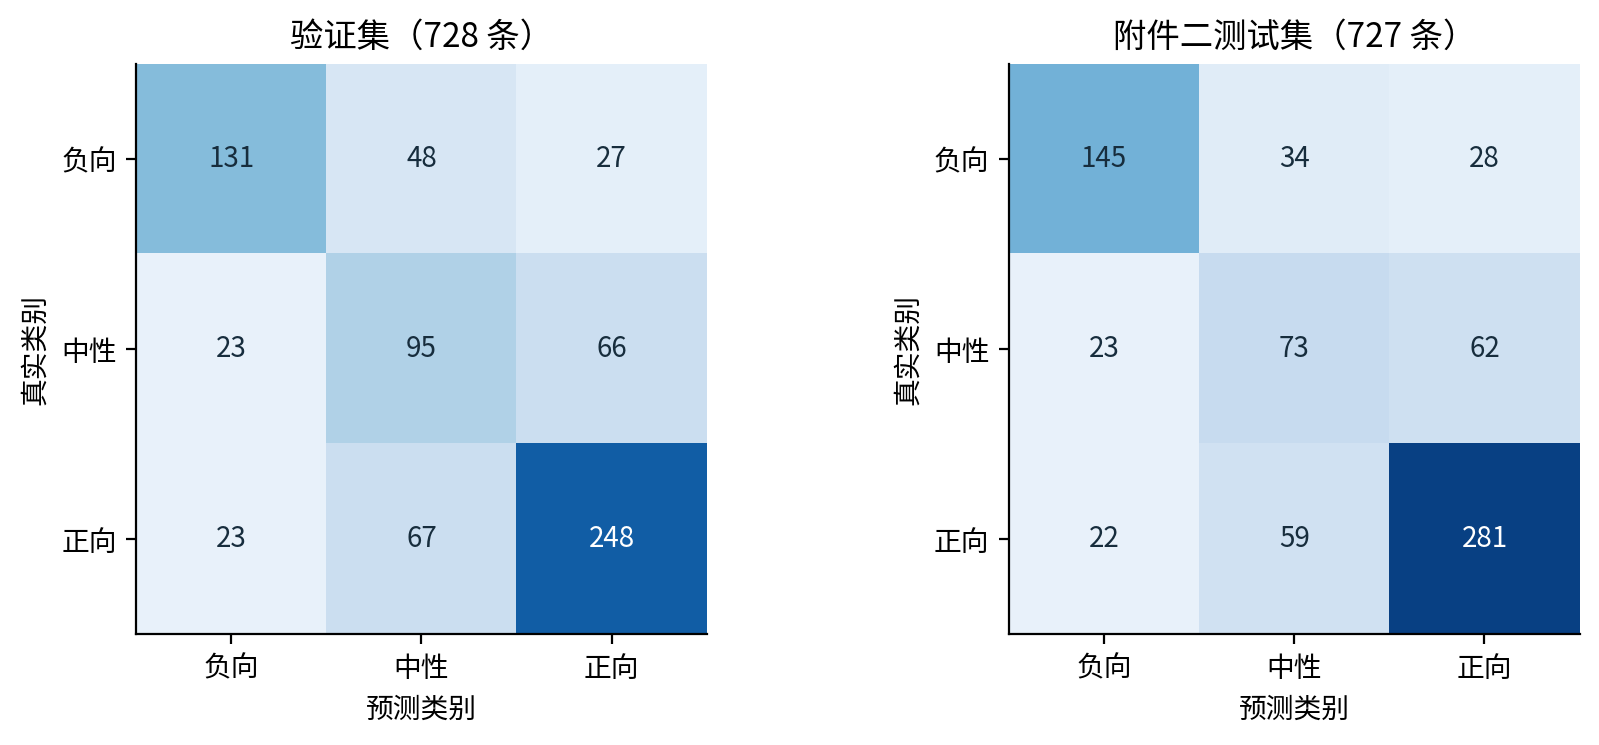
\includegraphics{../问题3/paper/figures/03_confusion.png}
\caption{三分类混淆矩阵，行是真值、列是预测。中性与正向之间的混淆较突出。\label{q3-fig4}}
\end{figure}

\begin{PaperTable}{5}

\begin{longtable}[]{@{}lllll@{}}
\caption{验证集逐类别性能\label{q3-tab7}}\tabularnewline
\toprule
\begin{minipage}[b]{0.17\columnwidth}\raggedright
验证类别\strut
\end{minipage} & \begin{minipage}[b]{0.17\columnwidth}\raggedright
Precision\strut
\end{minipage} & \begin{minipage}[b]{0.17\columnwidth}\raggedright
Recall\strut
\end{minipage} & \begin{minipage}[b]{0.17\columnwidth}\raggedright
F1\strut
\end{minipage} & \begin{minipage}[b]{0.17\columnwidth}\raggedright
支持数\strut
\end{minipage}\tabularnewline
\midrule
\endfirsthead
\caption[]{验证集逐类别性能（续）}\tabularnewline
\toprule
\begin{minipage}[b]{0.17\columnwidth}\raggedright
验证类别\strut
\end{minipage} & \begin{minipage}[b]{0.17\columnwidth}\raggedright
Precision\strut
\end{minipage} & \begin{minipage}[b]{0.17\columnwidth}\raggedright
Recall\strut
\end{minipage} & \begin{minipage}[b]{0.17\columnwidth}\raggedright
F1\strut
\end{minipage} & \begin{minipage}[b]{0.17\columnwidth}\raggedright
支持数\strut
\end{minipage}\tabularnewline
\midrule
\endhead
\begin{minipage}[t]{0.17\columnwidth}\raggedright
负向\strut
\end{minipage} & \begin{minipage}[t]{0.17\columnwidth}\raggedright
0.7401\strut
\end{minipage} & \begin{minipage}[t]{0.17\columnwidth}\raggedright
0.6359\strut
\end{minipage} & \begin{minipage}[t]{0.17\columnwidth}\raggedright
0.6841\strut
\end{minipage} & \begin{minipage}[t]{0.17\columnwidth}\raggedright
206\strut
\end{minipage}\tabularnewline
\begin{minipage}[t]{0.17\columnwidth}\raggedright
中性\strut
\end{minipage} & \begin{minipage}[t]{0.17\columnwidth}\raggedright
0.4524\strut
\end{minipage} & \begin{minipage}[t]{0.17\columnwidth}\raggedright
0.5163\strut
\end{minipage} & \begin{minipage}[t]{0.17\columnwidth}\raggedright
0.4822\strut
\end{minipage} & \begin{minipage}[t]{0.17\columnwidth}\raggedright
184\strut
\end{minipage}\tabularnewline
\begin{minipage}[t]{0.17\columnwidth}\raggedright
正向\strut
\end{minipage} & \begin{minipage}[t]{0.17\columnwidth}\raggedright
0.7273\strut
\end{minipage} & \begin{minipage}[t]{0.17\columnwidth}\raggedright
0.7337\strut
\end{minipage} & \begin{minipage}[t]{0.17\columnwidth}\raggedright
0.7305\strut
\end{minipage} & \begin{minipage}[t]{0.17\columnwidth}\raggedright
338\strut
\end{minipage}\tabularnewline
\bottomrule
\end{longtable}

\end{PaperTable}

\begin{figure}
\centering
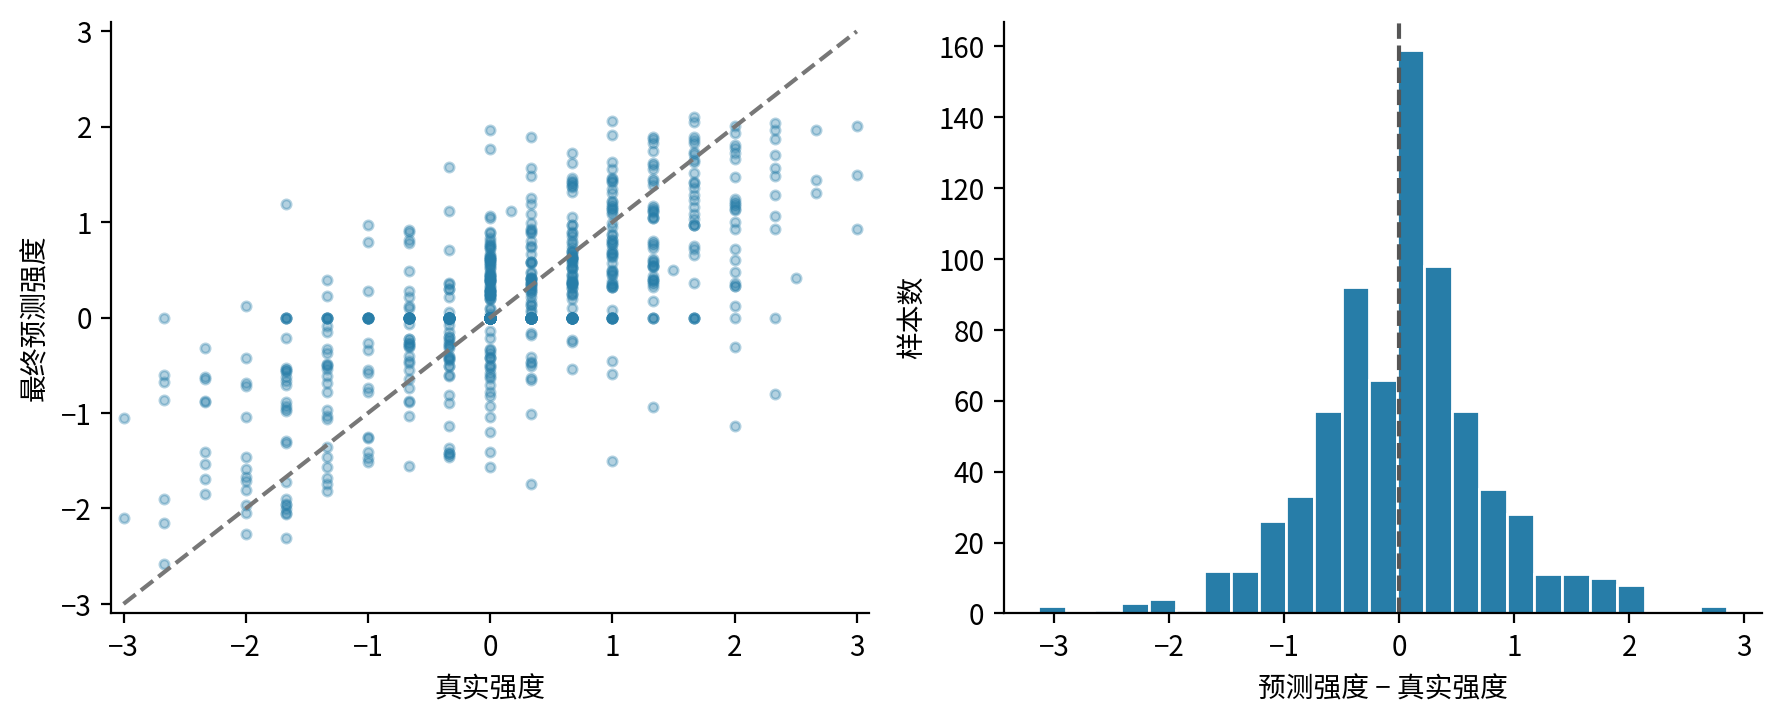
\includegraphics{../问题3/paper/figures/04_regression.png}
\caption{验证集最终强度散点与残差分布。预测中性置零，形成ŷ=0的水平带。\label{q3-fig5}}
\end{figure}

\hypertarget{q3-ux539fux751fux7ed3ux6784ux5bf9ux7167ux4e0eux6027ux80fdux53d6ux820d}{%
\subsubsection{原生结构对照与性能取舍}\label{q3-ux539fux751fux7ed3ux6784ux5bf9ux7167ux4e0eux6027ux80fdux53d6ux820d}}

在开源基线之外，补充原生骨干上``有序分类头''和``不确定性融合''两个模块的四格对照。四种设置均采用种子17、最多20轮、早停耐心4轮，以及相同的BERT学习率、其他层学习率、模态丢弃率和联合监督基础权重；各自按验证Macro-F1选择轮次和决策策略。有序分类头指可学习的累计阈值输出，与四种设置均保留的强度有序辅助损失不同。

\begin{PaperTable}{7}

\begin{longtable}[]{@{}lllllll@{}}
\caption{原生骨干的四种结构设置在验证集上的对照\label{q3-tab8}}\tabularnewline
\toprule
\begin{minipage}[b]{0.19\columnwidth}\raggedright
结构设置\strut
\end{minipage} & \begin{minipage}[b]{0.10\columnwidth}\raggedright
有序头\strut
\end{minipage} & \begin{minipage}[b]{0.10\columnwidth}\raggedright
不确定性\strut
\end{minipage} & \begin{minipage}[b]{0.10\columnwidth}\raggedright
轮次\strut
\end{minipage} & \begin{minipage}[b]{0.10\columnwidth}\raggedright
Acc(\%)\strut
\end{minipage} & \begin{minipage}[b]{0.10\columnwidth}\raggedright
Macro-F1\strut
\end{minipage} & \begin{minipage}[b]{0.10\columnwidth}\raggedright
MAE\strut
\end{minipage}\tabularnewline
\midrule
\endfirsthead
\caption[]{原生骨干的四种结构设置在验证集上的对照（续）}\tabularnewline
\toprule
\begin{minipage}[b]{0.19\columnwidth}\raggedright
结构设置\strut
\end{minipage} & \begin{minipage}[b]{0.10\columnwidth}\raggedright
有序头\strut
\end{minipage} & \begin{minipage}[b]{0.10\columnwidth}\raggedright
不确定性\strut
\end{minipage} & \begin{minipage}[b]{0.10\columnwidth}\raggedright
轮次\strut
\end{minipage} & \begin{minipage}[b]{0.10\columnwidth}\raggedright
Acc(\%)\strut
\end{minipage} & \begin{minipage}[b]{0.10\columnwidth}\raggedright
Macro-F1\strut
\end{minipage} & \begin{minipage}[b]{0.10\columnwidth}\raggedright
MAE\strut
\end{minipage}\tabularnewline
\midrule
\endhead
\begin{minipage}[t]{0.19\columnwidth}\raggedright
联合监督基础\strut
\end{minipage} & \begin{minipage}[t]{0.10\columnwidth}\raggedright
关\strut
\end{minipage} & \begin{minipage}[t]{0.10\columnwidth}\raggedright
关\strut
\end{minipage} & \begin{minipage}[t]{0.10\columnwidth}\raggedright
11\strut
\end{minipage} & \begin{minipage}[t]{0.10\columnwidth}\raggedright
65.25\strut
\end{minipage} & \begin{minipage}[t]{0.10\columnwidth}\raggedright
0.6412\strut
\end{minipage} & \begin{minipage}[t]{0.10\columnwidth}\raggedright
0.5578\strut
\end{minipage}\tabularnewline
\begin{minipage}[t]{0.19\columnwidth}\raggedright
仅有序分类头\strut
\end{minipage} & \begin{minipage}[t]{0.10\columnwidth}\raggedright
开\strut
\end{minipage} & \begin{minipage}[t]{0.10\columnwidth}\raggedright
关\strut
\end{minipage} & \begin{minipage}[t]{0.10\columnwidth}\raggedright
1\strut
\end{minipage} & \begin{minipage}[t]{0.10\columnwidth}\raggedright
63.46\strut
\end{minipage} & \begin{minipage}[t]{0.10\columnwidth}\raggedright
0.6230\strut
\end{minipage} & \begin{minipage}[t]{0.10\columnwidth}\raggedright
0.5706\strut
\end{minipage}\tabularnewline
\begin{minipage}[t]{0.19\columnwidth}\raggedright
有序头＋不确定性\strut
\end{minipage} & \begin{minipage}[t]{0.10\columnwidth}\raggedright
开\strut
\end{minipage} & \begin{minipage}[t]{0.10\columnwidth}\raggedright
开\strut
\end{minipage} & \begin{minipage}[t]{0.10\columnwidth}\raggedright
3\strut
\end{minipage} & \begin{minipage}[t]{0.10\columnwidth}\raggedright
63.74\strut
\end{minipage} & \begin{minipage}[t]{0.10\columnwidth}\raggedright
0.6165\strut
\end{minipage} & \begin{minipage}[t]{0.10\columnwidth}\raggedright
0.5688\strut
\end{minipage}\tabularnewline
\begin{minipage}[t]{0.19\columnwidth}\raggedright
不确定性融合（主）\strut
\end{minipage} & \begin{minipage}[t]{0.10\columnwidth}\raggedright
关\strut
\end{minipage} & \begin{minipage}[t]{0.10\columnwidth}\raggedright
开\strut
\end{minipage} & \begin{minipage}[t]{0.10\columnwidth}\raggedright
5\strut
\end{minipage} & \begin{minipage}[t]{0.10\columnwidth}\raggedright
65.11\strut
\end{minipage} & \begin{minipage}[t]{0.10\columnwidth}\raggedright
0.6323\strut
\end{minipage} & \begin{minipage}[t]{0.10\columnwidth}\raggedright
0.5397\strut
\end{minipage}\tabularnewline
\bottomrule
\end{longtable}

\end{PaperTable}

仅加入有序分类头时，验证Macro-F1为0.6230、MAE为0.5706；同时加入有序头与不确定性时，相应为0.6165和0.5688，均弱于本文主模型的0.6323和0.5397。对应的既有冻结测试结果中，两种有序设置的准确率均为66.02\%，Macro-F1分别为0.6342和0.6212，MAE分别为0.6210和0.6184，也未优于主模型。由此可见，更强的输出约束或更多融合模块并不自动带来更好的分类与回归表现。

联合监督基础设置在验证集的Macro-F1为0.6412，高于主模型；主模型的MAE则降低约0.0181。因此，四格对照支持不同结构之间存在性能取舍，不能据其中两个较弱设置宣称不确定性模块对所有指标均有增益。各设置使用各自验证最优策略，比较包含训练与策略选择的共同影响；单种子结果也不构成稳定提升的证据。

\hypertarget{q3-ux5b66ux4e60ux7387ux6210ux7ec4ux5bf9ux7167ux4e0eux8f83ux5f31ux914dux7f6eux5206ux6790}{%
\subsubsection{学习率成组对照与较弱配置分析}\label{q3-ux5b66ux4e60ux7387ux6210ux7ec4ux5bf9ux7167ux4e0eux8f83ux5f31ux914dux7f6eux5206ux6790}}

\hypertarget{q3-ux9a8cux8bc1ux96c6ux9519ux8befux5f52ux56e0}{%
\subsubsection{验证集错误归因}\label{q3-ux9a8cux8bc1ux96c6ux9519ux8befux5f52ux56e0}}

验证集728条中分类错误254条。真实中性的184条中，89条被判为非中性（23条负向、66条正向），中性召回率51.63\%；真实正向338条中67条被判中性，真实负向206条中48条被判中性。中性与正向混淆构成主要误差来源。中性边界校准改善取舍，仍不能解决说明性文本、弱情感与标注差异；继续扩大偏置会同时改变正负样本被归零的比例。

\begin{PaperTable}{5}

\begin{longtable}[]{@{}lllll@{}}
\caption{验证集标签与观测分组的误差\label{q3-tab12}}\tabularnewline
\toprule
\begin{minipage}[b]{0.25\columnwidth}\raggedright
验证分组\strut
\end{minipage} & \begin{minipage}[b]{0.15\columnwidth}\raggedright
样本数\strut
\end{minipage} & \begin{minipage}[b]{0.15\columnwidth}\raggedright
分类错误数\strut
\end{minipage} & \begin{minipage}[b]{0.15\columnwidth}\raggedright
错误率\strut
\end{minipage} & \begin{minipage}[b]{0.15\columnwidth}\raggedright
最终MAE\strut
\end{minipage}\tabularnewline
\midrule
\endfirsthead
\caption[]{验证集标签与观测分组的误差（续）}\tabularnewline
\toprule
\begin{minipage}[b]{0.25\columnwidth}\raggedright
验证分组\strut
\end{minipage} & \begin{minipage}[b]{0.15\columnwidth}\raggedright
样本数\strut
\end{minipage} & \begin{minipage}[b]{0.15\columnwidth}\raggedright
分类错误数\strut
\end{minipage} & \begin{minipage}[b]{0.15\columnwidth}\raggedright
错误率\strut
\end{minipage} & \begin{minipage}[b]{0.15\columnwidth}\raggedright
最终MAE\strut
\end{minipage}\tabularnewline
\midrule
\endhead
\begin{minipage}[t]{0.25\columnwidth}\raggedright
真实负向\strut
\end{minipage} & \begin{minipage}[t]{0.15\columnwidth}\raggedright
206\strut
\end{minipage} & \begin{minipage}[t]{0.15\columnwidth}\raggedright
75\strut
\end{minipage} & \begin{minipage}[t]{0.15\columnwidth}\raggedright
36.41\%\strut
\end{minipage} & \begin{minipage}[t]{0.15\columnwidth}\raggedright
0.7233\strut
\end{minipage}\tabularnewline
\begin{minipage}[t]{0.25\columnwidth}\raggedright
真实中性\strut
\end{minipage} & \begin{minipage}[t]{0.15\columnwidth}\raggedright
184\strut
\end{minipage} & \begin{minipage}[t]{0.15\columnwidth}\raggedright
89\strut
\end{minipage} & \begin{minipage}[t]{0.15\columnwidth}\raggedright
48.37\%\strut
\end{minipage} & \begin{minipage}[t]{0.15\columnwidth}\raggedright
0.2580\strut
\end{minipage}\tabularnewline
\begin{minipage}[t]{0.25\columnwidth}\raggedright
真实正向\strut
\end{minipage} & \begin{minipage}[t]{0.15\columnwidth}\raggedright
338\strut
\end{minipage} & \begin{minipage}[t]{0.15\columnwidth}\raggedright
90\strut
\end{minipage} & \begin{minipage}[t]{0.15\columnwidth}\raggedright
26.63\%\strut
\end{minipage} & \begin{minipage}[t]{0.15\columnwidth}\raggedright
0.5811\strut
\end{minipage}\tabularnewline
\begin{minipage}[t]{0.25\columnwidth}\raggedright
视觉无有效观测\strut
\end{minipage} & \begin{minipage}[t]{0.15\columnwidth}\raggedright
15\strut
\end{minipage} & \begin{minipage}[t]{0.15\columnwidth}\raggedright
6\strut
\end{minipage} & \begin{minipage}[t]{0.15\columnwidth}\raggedright
40.00\%\strut
\end{minipage} & \begin{minipage}[t]{0.15\columnwidth}\raggedright
0.4789\strut
\end{minipage}\tabularnewline
\begin{minipage}[t]{0.25\columnwidth}\raggedright
视觉存在有效观测\strut
\end{minipage} & \begin{minipage}[t]{0.15\columnwidth}\raggedright
713\strut
\end{minipage} & \begin{minipage}[t]{0.15\columnwidth}\raggedright
248\strut
\end{minipage} & \begin{minipage}[t]{0.15\columnwidth}\raggedright
34.78\%\strut
\end{minipage} & \begin{minipage}[t]{0.15\columnwidth}\raggedright
0.5410\strut
\end{minipage}\tabularnewline
\bottomrule
\end{longtable}

\end{PaperTable}

分组差异同时受标签分布、语句内容和观测质量影响，只能作为错误诊断线索，不构成模态缺失的因果效应。分类贡献在文本上的集中说明模型更依赖语言判别；语音与视觉的较低分类净贡献也可能来自内部正负项抵消，不能视为它们没有可用信息。强度预测的收缩与中性归零会对强情感样本产生较大残差，图\ref{q3-fig5}可用于检查这种系统偏差。

\hypertarget{q3-ux89e3ux91caux5b8cux5907ux6027ux68c0ux9a8c}{%
\subsubsection{解释完备性检验}\label{q3-ux89e3ux91caux5b8cux5907ux6027ux68c0ux9a8c}}

\begin{PaperTable}{4}

\begin{longtable}[]{@{}llll@{}}
\caption{分类间隔与回归预激活的分解误差\label{q3-tab13}}\tabularnewline
\toprule
\begin{minipage}[b]{0.35\columnwidth}\raggedright
解释检查\strut
\end{minipage} & \begin{minipage}[b]{0.18\columnwidth}\raggedright
验证\strut
\end{minipage} & \begin{minipage}[b]{0.18\columnwidth}\raggedright
测试\strut
\end{minipage} & \begin{minipage}[b]{0.18\columnwidth}\raggedright
附件4\strut
\end{minipage}\tabularnewline
\midrule
\endfirsthead
\caption[]{分类间隔与回归预激活的分解误差（续）}\tabularnewline
\toprule
\begin{minipage}[b]{0.35\columnwidth}\raggedright
解释检查\strut
\end{minipage} & \begin{minipage}[b]{0.18\columnwidth}\raggedright
验证\strut
\end{minipage} & \begin{minipage}[b]{0.18\columnwidth}\raggedright
测试\strut
\end{minipage} & \begin{minipage}[b]{0.18\columnwidth}\raggedright
附件4\strut
\end{minipage}\tabularnewline
\midrule
\endhead
\begin{minipage}[t]{0.35\columnwidth}\raggedright
分类间隔最大核算误差\strut
\end{minipage} & \begin{minipage}[t]{0.18\columnwidth}\raggedright
1.52e-06\strut
\end{minipage} & \begin{minipage}[t]{0.18\columnwidth}\raggedright
1.52e-06\strut
\end{minipage} & \begin{minipage}[t]{0.18\columnwidth}\raggedright
5.29e-07\strut
\end{minipage}\tabularnewline
\begin{minipage}[t]{0.35\columnwidth}\raggedright
回归q最大核算误差\strut
\end{minipage} & \begin{minipage}[t]{0.18\columnwidth}\raggedright
1.53e-07\strut
\end{minipage} & \begin{minipage}[t]{0.18\columnwidth}\raggedright
1.53e-07\strut
\end{minipage} & \begin{minipage}[t]{0.18\columnwidth}\raggedright
3.35e-08\strut
\end{minipage}\tabularnewline
\begin{minipage}[t]{0.35\columnwidth}\raggedright
逐样本核查数量\strut
\end{minipage} & \begin{minipage}[t]{0.18\columnwidth}\raggedright
728\strut
\end{minipage} & \begin{minipage}[t]{0.18\columnwidth}\raggedright
727\strut
\end{minipage} & \begin{minipage}[t]{0.18\columnwidth}\raggedright
20\strut
\end{minipage}\tabularnewline
\bottomrule
\end{longtable}

\end{PaperTable}

将三模态净分数与偏置相加，并与同次前向的目标分数逐条比较。1475条样本的分解误差均处于浮点计算误差范围。该检查说明解释忠实于当前读出的数值，不证明某个证据词是人类情感成因。本主模型没有单独完成随机扰动对照、多种子解释稳定性或人类证据标注评价，局部读出核算与输入扰动忠实性仍需分别检验。

\hypertarget{q3-ux4e09ux6a21ux6001ux4f5cux7528ux5deeux5f02ux4e0eux5c40ux90e8ux91cdux8981ux6027}{%
\subsection{三模态作用差异与局部重要性}\label{q3-ux4e09ux6a21ux6001ux4f5cux7528ux5deeux5f02ux4e0eux5c40ux90e8ux91cdux8981ux6027}}

\hypertarget{q3-ux5206ux7c7bux56deux5f52ux4e0eux53efux9760ux6027ux7684ux533aux522b}{%
\subsubsection{分类、回归与可靠性的区别}\label{q3-ux5206ux7c7bux56deux5f52ux4e0eux53efux9760ux6027ux7684ux533aux522b}}

\begin{PaperTable}{4}

\begin{longtable}[]{@{}llll@{}}
\caption{三模态净贡献占比的样本均值\label{q3-tab14}}\tabularnewline
\toprule
\begin{minipage}[b]{0.36\columnwidth}\raggedright
集合/解释目标\strut
\end{minipage} & \begin{minipage}[b]{0.17\columnwidth}\raggedright
文本(\%)\strut
\end{minipage} & \begin{minipage}[b]{0.17\columnwidth}\raggedright
语音(\%)\strut
\end{minipage} & \begin{minipage}[b]{0.17\columnwidth}\raggedright
视觉(\%)\strut
\end{minipage}\tabularnewline
\midrule
\endfirsthead
\caption[]{三模态净贡献占比的样本均值（续）}\tabularnewline
\toprule
\begin{minipage}[b]{0.36\columnwidth}\raggedright
集合/解释目标\strut
\end{minipage} & \begin{minipage}[b]{0.17\columnwidth}\raggedright
文本(\%)\strut
\end{minipage} & \begin{minipage}[b]{0.17\columnwidth}\raggedright
语音(\%)\strut
\end{minipage} & \begin{minipage}[b]{0.17\columnwidth}\raggedright
视觉(\%)\strut
\end{minipage}\tabularnewline
\midrule
\endhead
\begin{minipage}[t]{0.36\columnwidth}\raggedright
验证集/分类间隔\strut
\end{minipage} & \begin{minipage}[t]{0.17\columnwidth}\raggedright
84.76\strut
\end{minipage} & \begin{minipage}[t]{0.17\columnwidth}\raggedright
6.88\strut
\end{minipage} & \begin{minipage}[t]{0.17\columnwidth}\raggedright
8.36\strut
\end{minipage}\tabularnewline
\begin{minipage}[t]{0.36\columnwidth}\raggedright
验证集/回归q\strut
\end{minipage} & \begin{minipage}[t]{0.17\columnwidth}\raggedright
68.16\strut
\end{minipage} & \begin{minipage}[t]{0.17\columnwidth}\raggedright
15.98\strut
\end{minipage} & \begin{minipage}[t]{0.17\columnwidth}\raggedright
15.86\strut
\end{minipage}\tabularnewline
\begin{minipage}[t]{0.36\columnwidth}\raggedright
附件二测试集/分类间隔\strut
\end{minipage} & \begin{minipage}[t]{0.17\columnwidth}\raggedright
84.62\strut
\end{minipage} & \begin{minipage}[t]{0.17\columnwidth}\raggedright
6.71\strut
\end{minipage} & \begin{minipage}[t]{0.17\columnwidth}\raggedright
8.68\strut
\end{minipage}\tabularnewline
\begin{minipage}[t]{0.36\columnwidth}\raggedright
附件二测试集/回归q\strut
\end{minipage} & \begin{minipage}[t]{0.17\columnwidth}\raggedright
71.14\strut
\end{minipage} & \begin{minipage}[t]{0.17\columnwidth}\raggedright
13.58\strut
\end{minipage} & \begin{minipage}[t]{0.17\columnwidth}\raggedright
15.28\strut
\end{minipage}\tabularnewline
\bottomrule
\end{longtable}

\end{PaperTable}

上述比例先在每条样本内归一化，再对样本等权平均。验证与测试的分类文本占比均约85\%，而回归文本占比约68\%---71\%，语音和视觉对强度的作用相对更高。附件4分类主要参考模态为文本20/20，回归主要模态为文本18/20、视觉2/20（02、14）；02与14的视觉回归净贡献占比分别为48.12\%与41.09\%。因此``分类主要看文本''不能推导出``强度估计中的视觉无作用''。

\begin{figure}
\centering
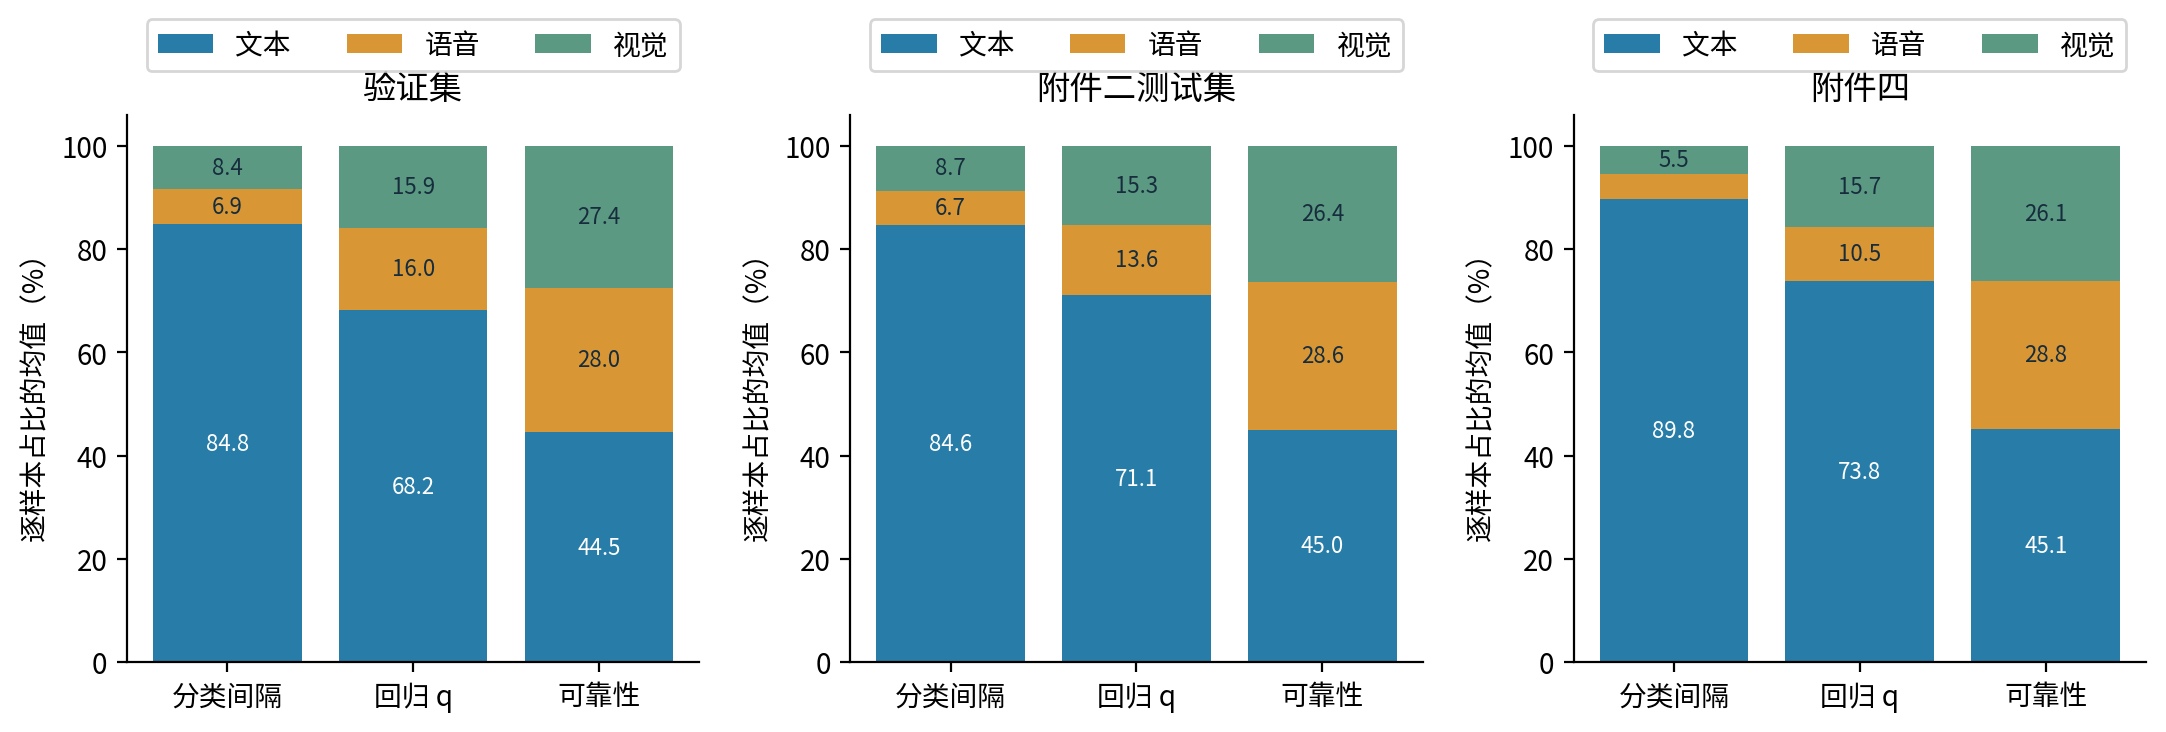
\includegraphics{../问题3/paper/figures/05_contributions.png}
\caption{分类贡献、回归贡献与可靠性权重的对照。三者解释不同对象，不能互换。\label{q3-fig7}}
\end{figure}

附件4平均可靠性权重T/A/V为45.07\%/28.80\%/26.12\%，分类净贡献却为89.78\%/4.71\%/5.51\%。这来自不同模态证据大小、方向和抵消程度的共同影响，表明直接把可靠性权重写成贡献会失真。附件4的13号视觉数组全部为零，视觉单项和交互关闭，其视觉贡献应为0；验证和测试分别有15、28条视觉无有效数值观测。

\hypertarget{q3-ux4e3bux8981ux53c2ux8003ux6a21ux6001ux5185ux7684ux5c40ux90e8ux8bc1ux636eux5206ux5e03}{%
\subsubsection{主要参考模态内的局部证据分布}\label{q3-ux4e3bux8981ux53c2ux8003ux6a21ux6001ux5185ux7684ux5c40ux90e8ux8bc1ux636eux5206ux5e03}}

局部重要性按分类间隔的有符号读出绘制。为避免只呈现支持结论的片段，图中保留每个有效位置及其正负方向：蓝色为支持预测类，红色为反对预测类。横轴采用原始分数量纲，纵轴保留原BERT位置与原文词元；这使典型解释可以回查到输入，而不只给出无位置的模态占比。

\begin{figure}
\centering
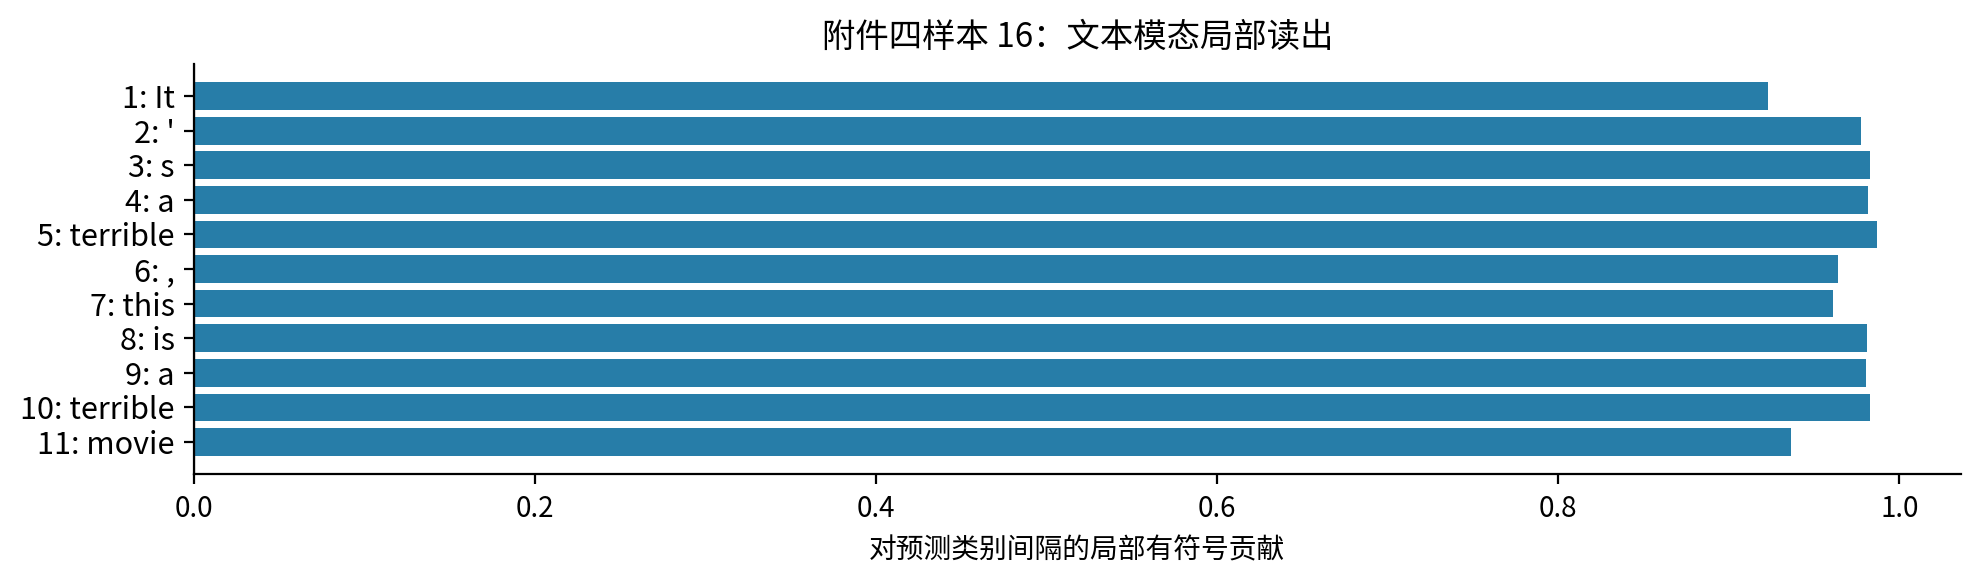
\includegraphics{../问题3/paper/figures/06_local_16.png}
\caption{附件4样本16的主要参考模态内局部重要性。每行给出原BERT位置和对应原文，负值表示反对当前类别间隔；词的上下文由BERT编码。\label{q3-fig8}}
\end{figure}

\hypertarget{q3-ux9644ux4ef6ux56dbux5168ux91cfux9884ux6d4bux4e0eux5178ux578bux89e3ux91ca}{%
\subsection{附件四全量预测与典型解释}\label{q3-ux9644ux4ef6ux56dbux5168ux91cfux9884ux6d4bux4e0eux5178ux578bux89e3ux91ca}}

\hypertarget{q3-ux5168ux91cfux9884ux6d4bux4e0eux4e09ux6a21ux6001ux4f5cux7528ux7a0bux5ea6}{%
\subsubsection{全量预测与三模态作用程度}\label{q3-ux5168ux91cfux9884ux6d4bux4e0eux4e09ux6a21ux6001ux4f5cux7528ux7a0bux5ea6}}

附件四按题目中的无标签专项集处理。表中给出全部20条样本的预测极性、最终强度、分类间隔的三模态净贡献占比及分类、回归主要参考模态。比例均由同次前向的有符号净分数取绝对值后归一化；少量行因四舍五入可能不恰好合计100\%。

\begin{PaperTable}{7}

\begin{longtable}[]{@{}lllllll@{}}
\caption{附件四20条样本的预测与分类贡献汇总\label{q3-tab15}}\tabularnewline
\toprule
\begin{minipage}[b]{0.06\columnwidth}\raggedright
编号\strut
\end{minipage} & \begin{minipage}[b]{0.11\columnwidth}\raggedright
预测极性\strut
\end{minipage} & \begin{minipage}[b]{0.16\columnwidth}\raggedright
最终强度\strut
\end{minipage} & \begin{minipage}[b]{0.11\columnwidth}\raggedright
文本(\%)\strut
\end{minipage} & \begin{minipage}[b]{0.11\columnwidth}\raggedright
语音(\%)\strut
\end{minipage} & \begin{minipage}[b]{0.11\columnwidth}\raggedright
视觉(\%)\strut
\end{minipage} & \begin{minipage}[b]{0.16\columnwidth}\raggedright
分类/回归主模态\strut
\end{minipage}\tabularnewline
\midrule
\endfirsthead
\caption[]{附件四20条样本的预测与分类贡献汇总（续）}\tabularnewline
\toprule
\begin{minipage}[b]{0.06\columnwidth}\raggedright
编号\strut
\end{minipage} & \begin{minipage}[b]{0.11\columnwidth}\raggedright
预测极性\strut
\end{minipage} & \begin{minipage}[b]{0.16\columnwidth}\raggedright
最终强度\strut
\end{minipage} & \begin{minipage}[b]{0.11\columnwidth}\raggedright
文本(\%)\strut
\end{minipage} & \begin{minipage}[b]{0.11\columnwidth}\raggedright
语音(\%)\strut
\end{minipage} & \begin{minipage}[b]{0.11\columnwidth}\raggedright
视觉(\%)\strut
\end{minipage} & \begin{minipage}[b]{0.16\columnwidth}\raggedright
分类/回归主模态\strut
\end{minipage}\tabularnewline
\midrule
\endhead
\begin{minipage}[t]{0.06\columnwidth}\raggedright
01\strut
\end{minipage} & \begin{minipage}[t]{0.11\columnwidth}\raggedright
中性\strut
\end{minipage} & \begin{minipage}[t]{0.16\columnwidth}\raggedright
+0.0000\strut
\end{minipage} & \begin{minipage}[t]{0.11\columnwidth}\raggedright
96.43\strut
\end{minipage} & \begin{minipage}[t]{0.11\columnwidth}\raggedright
3.50\strut
\end{minipage} & \begin{minipage}[t]{0.11\columnwidth}\raggedright
0.06\strut
\end{minipage} & \begin{minipage}[t]{0.16\columnwidth}\raggedright
T/T\strut
\end{minipage}\tabularnewline
\begin{minipage}[t]{0.06\columnwidth}\raggedright
02\strut
\end{minipage} & \begin{minipage}[t]{0.11\columnwidth}\raggedright
正向\strut
\end{minipage} & \begin{minipage}[t]{0.16\columnwidth}\raggedright
+1.0e-06\strut
\end{minipage} & \begin{minipage}[t]{0.11\columnwidth}\raggedright
74.42\strut
\end{minipage} & \begin{minipage}[t]{0.11\columnwidth}\raggedright
22.81\strut
\end{minipage} & \begin{minipage}[t]{0.11\columnwidth}\raggedright
2.76\strut
\end{minipage} & \begin{minipage}[t]{0.16\columnwidth}\raggedright
T/V\strut
\end{minipage}\tabularnewline
\begin{minipage}[t]{0.06\columnwidth}\raggedright
03\strut
\end{minipage} & \begin{minipage}[t]{0.11\columnwidth}\raggedright
负向\strut
\end{minipage} & \begin{minipage}[t]{0.16\columnwidth}\raggedright
-0.6588\strut
\end{minipage} & \begin{minipage}[t]{0.11\columnwidth}\raggedright
98.46\strut
\end{minipage} & \begin{minipage}[t]{0.11\columnwidth}\raggedright
0.41\strut
\end{minipage} & \begin{minipage}[t]{0.11\columnwidth}\raggedright
1.13\strut
\end{minipage} & \begin{minipage}[t]{0.16\columnwidth}\raggedright
T/T\strut
\end{minipage}\tabularnewline
\begin{minipage}[t]{0.06\columnwidth}\raggedright
04\strut
\end{minipage} & \begin{minipage}[t]{0.11\columnwidth}\raggedright
负向\strut
\end{minipage} & \begin{minipage}[t]{0.16\columnwidth}\raggedright
-0.4144\strut
\end{minipage} & \begin{minipage}[t]{0.11\columnwidth}\raggedright
98.67\strut
\end{minipage} & \begin{minipage}[t]{0.11\columnwidth}\raggedright
0.31\strut
\end{minipage} & \begin{minipage}[t]{0.11\columnwidth}\raggedright
1.02\strut
\end{minipage} & \begin{minipage}[t]{0.16\columnwidth}\raggedright
T/T\strut
\end{minipage}\tabularnewline
\begin{minipage}[t]{0.06\columnwidth}\raggedright
05\strut
\end{minipage} & \begin{minipage}[t]{0.11\columnwidth}\raggedright
正向\strut
\end{minipage} & \begin{minipage}[t]{0.16\columnwidth}\raggedright
+0.7983\strut
\end{minipage} & \begin{minipage}[t]{0.11\columnwidth}\raggedright
81.97\strut
\end{minipage} & \begin{minipage}[t]{0.11\columnwidth}\raggedright
3.64\strut
\end{minipage} & \begin{minipage}[t]{0.11\columnwidth}\raggedright
14.38\strut
\end{minipage} & \begin{minipage}[t]{0.16\columnwidth}\raggedright
T/T\strut
\end{minipage}\tabularnewline
\begin{minipage}[t]{0.06\columnwidth}\raggedright
06\strut
\end{minipage} & \begin{minipage}[t]{0.11\columnwidth}\raggedright
正向\strut
\end{minipage} & \begin{minipage}[t]{0.16\columnwidth}\raggedright
+0.9139\strut
\end{minipage} & \begin{minipage}[t]{0.11\columnwidth}\raggedright
93.60\strut
\end{minipage} & \begin{minipage}[t]{0.11\columnwidth}\raggedright
3.66\strut
\end{minipage} & \begin{minipage}[t]{0.11\columnwidth}\raggedright
2.74\strut
\end{minipage} & \begin{minipage}[t]{0.16\columnwidth}\raggedright
T/T\strut
\end{minipage}\tabularnewline
\begin{minipage}[t]{0.06\columnwidth}\raggedright
07\strut
\end{minipage} & \begin{minipage}[t]{0.11\columnwidth}\raggedright
正向\strut
\end{minipage} & \begin{minipage}[t]{0.16\columnwidth}\raggedright
+0.8535\strut
\end{minipage} & \begin{minipage}[t]{0.11\columnwidth}\raggedright
90.50\strut
\end{minipage} & \begin{minipage}[t]{0.11\columnwidth}\raggedright
2.19\strut
\end{minipage} & \begin{minipage}[t]{0.11\columnwidth}\raggedright
7.31\strut
\end{minipage} & \begin{minipage}[t]{0.16\columnwidth}\raggedright
T/T\strut
\end{minipage}\tabularnewline
\begin{minipage}[t]{0.06\columnwidth}\raggedright
08\strut
\end{minipage} & \begin{minipage}[t]{0.11\columnwidth}\raggedright
正向\strut
\end{minipage} & \begin{minipage}[t]{0.16\columnwidth}\raggedright
+0.5174\strut
\end{minipage} & \begin{minipage}[t]{0.11\columnwidth}\raggedright
98.47\strut
\end{minipage} & \begin{minipage}[t]{0.11\columnwidth}\raggedright
0.46\strut
\end{minipage} & \begin{minipage}[t]{0.11\columnwidth}\raggedright
1.07\strut
\end{minipage} & \begin{minipage}[t]{0.16\columnwidth}\raggedright
T/T\strut
\end{minipage}\tabularnewline
\begin{minipage}[t]{0.06\columnwidth}\raggedright
09\strut
\end{minipage} & \begin{minipage}[t]{0.11\columnwidth}\raggedright
负向\strut
\end{minipage} & \begin{minipage}[t]{0.16\columnwidth}\raggedright
-2.2932\strut
\end{minipage} & \begin{minipage}[t]{0.11\columnwidth}\raggedright
99.50\strut
\end{minipage} & \begin{minipage}[t]{0.11\columnwidth}\raggedright
0.19\strut
\end{minipage} & \begin{minipage}[t]{0.11\columnwidth}\raggedright
0.31\strut
\end{minipage} & \begin{minipage}[t]{0.16\columnwidth}\raggedright
T/T\strut
\end{minipage}\tabularnewline
\begin{minipage}[t]{0.06\columnwidth}\raggedright
10\strut
\end{minipage} & \begin{minipage}[t]{0.11\columnwidth}\raggedright
负向\strut
\end{minipage} & \begin{minipage}[t]{0.16\columnwidth}\raggedright
-2.1598\strut
\end{minipage} & \begin{minipage}[t]{0.11\columnwidth}\raggedright
99.37\strut
\end{minipage} & \begin{minipage}[t]{0.11\columnwidth}\raggedright
0.63\strut
\end{minipage} & \begin{minipage}[t]{0.11\columnwidth}\raggedright
0.01\strut
\end{minipage} & \begin{minipage}[t]{0.16\columnwidth}\raggedright
T/T\strut
\end{minipage}\tabularnewline
\begin{minipage}[t]{0.06\columnwidth}\raggedright
11\strut
\end{minipage} & \begin{minipage}[t]{0.11\columnwidth}\raggedright
负向\strut
\end{minipage} & \begin{minipage}[t]{0.16\columnwidth}\raggedright
-1.7402\strut
\end{minipage} & \begin{minipage}[t]{0.11\columnwidth}\raggedright
99.40\strut
\end{minipage} & \begin{minipage}[t]{0.11\columnwidth}\raggedright
0.52\strut
\end{minipage} & \begin{minipage}[t]{0.11\columnwidth}\raggedright
0.08\strut
\end{minipage} & \begin{minipage}[t]{0.16\columnwidth}\raggedright
T/T\strut
\end{minipage}\tabularnewline
\begin{minipage}[t]{0.06\columnwidth}\raggedright
12\strut
\end{minipage} & \begin{minipage}[t]{0.11\columnwidth}\raggedright
负向\strut
\end{minipage} & \begin{minipage}[t]{0.16\columnwidth}\raggedright
-0.6896\strut
\end{minipage} & \begin{minipage}[t]{0.11\columnwidth}\raggedright
96.60\strut
\end{minipage} & \begin{minipage}[t]{0.11\columnwidth}\raggedright
2.59\strut
\end{minipage} & \begin{minipage}[t]{0.11\columnwidth}\raggedright
0.81\strut
\end{minipage} & \begin{minipage}[t]{0.16\columnwidth}\raggedright
T/T\strut
\end{minipage}\tabularnewline
\begin{minipage}[t]{0.06\columnwidth}\raggedright
13\strut
\end{minipage} & \begin{minipage}[t]{0.11\columnwidth}\raggedright
中性\strut
\end{minipage} & \begin{minipage}[t]{0.16\columnwidth}\raggedright
+0.0000\strut
\end{minipage} & \begin{minipage}[t]{0.11\columnwidth}\raggedright
93.27\strut
\end{minipage} & \begin{minipage}[t]{0.11\columnwidth}\raggedright
6.73\strut
\end{minipage} & \begin{minipage}[t]{0.11\columnwidth}\raggedright
0.00\strut
\end{minipage} & \begin{minipage}[t]{0.16\columnwidth}\raggedright
T/T\strut
\end{minipage}\tabularnewline
\begin{minipage}[t]{0.06\columnwidth}\raggedright
14\strut
\end{minipage} & \begin{minipage}[t]{0.11\columnwidth}\raggedright
中性\strut
\end{minipage} & \begin{minipage}[t]{0.16\columnwidth}\raggedright
+0.0000\strut
\end{minipage} & \begin{minipage}[t]{0.11\columnwidth}\raggedright
80.66\strut
\end{minipage} & \begin{minipage}[t]{0.11\columnwidth}\raggedright
4.35\strut
\end{minipage} & \begin{minipage}[t]{0.11\columnwidth}\raggedright
14.99\strut
\end{minipage} & \begin{minipage}[t]{0.16\columnwidth}\raggedright
T/V\strut
\end{minipage}\tabularnewline
\begin{minipage}[t]{0.06\columnwidth}\raggedright
15\strut
\end{minipage} & \begin{minipage}[t]{0.11\columnwidth}\raggedright
正向\strut
\end{minipage} & \begin{minipage}[t]{0.16\columnwidth}\raggedright
+0.6387\strut
\end{minipage} & \begin{minipage}[t]{0.11\columnwidth}\raggedright
73.61\strut
\end{minipage} & \begin{minipage}[t]{0.11\columnwidth}\raggedright
15.05\strut
\end{minipage} & \begin{minipage}[t]{0.11\columnwidth}\raggedright
11.34\strut
\end{minipage} & \begin{minipage}[t]{0.16\columnwidth}\raggedright
T/T\strut
\end{minipage}\tabularnewline
\begin{minipage}[t]{0.06\columnwidth}\raggedright
16\strut
\end{minipage} & \begin{minipage}[t]{0.11\columnwidth}\raggedright
负向\strut
\end{minipage} & \begin{minipage}[t]{0.16\columnwidth}\raggedright
-2.6363\strut
\end{minipage} & \begin{minipage}[t]{0.11\columnwidth}\raggedright
99.04\strut
\end{minipage} & \begin{minipage}[t]{0.11\columnwidth}\raggedright
0.01\strut
\end{minipage} & \begin{minipage}[t]{0.11\columnwidth}\raggedright
0.95\strut
\end{minipage} & \begin{minipage}[t]{0.16\columnwidth}\raggedright
T/T\strut
\end{minipage}\tabularnewline
\begin{minipage}[t]{0.06\columnwidth}\raggedright
17\strut
\end{minipage} & \begin{minipage}[t]{0.11\columnwidth}\raggedright
正向\strut
\end{minipage} & \begin{minipage}[t]{0.16\columnwidth}\raggedright
+1.7645\strut
\end{minipage} & \begin{minipage}[t]{0.11\columnwidth}\raggedright
94.11\strut
\end{minipage} & \begin{minipage}[t]{0.11\columnwidth}\raggedright
1.66\strut
\end{minipage} & \begin{minipage}[t]{0.11\columnwidth}\raggedright
4.23\strut
\end{minipage} & \begin{minipage}[t]{0.16\columnwidth}\raggedright
T/T\strut
\end{minipage}\tabularnewline
\begin{minipage}[t]{0.06\columnwidth}\raggedright
18\strut
\end{minipage} & \begin{minipage}[t]{0.11\columnwidth}\raggedright
负向\strut
\end{minipage} & \begin{minipage}[t]{0.16\columnwidth}\raggedright
-0.5241\strut
\end{minipage} & \begin{minipage}[t]{0.11\columnwidth}\raggedright
93.28\strut
\end{minipage} & \begin{minipage}[t]{0.11\columnwidth}\raggedright
0.09\strut
\end{minipage} & \begin{minipage}[t]{0.11\columnwidth}\raggedright
6.63\strut
\end{minipage} & \begin{minipage}[t]{0.16\columnwidth}\raggedright
T/T\strut
\end{minipage}\tabularnewline
\begin{minipage}[t]{0.06\columnwidth}\raggedright
19\strut
\end{minipage} & \begin{minipage}[t]{0.11\columnwidth}\raggedright
正向\strut
\end{minipage} & \begin{minipage}[t]{0.16\columnwidth}\raggedright
+0.6309\strut
\end{minipage} & \begin{minipage}[t]{0.11\columnwidth}\raggedright
71.34\strut
\end{minipage} & \begin{minipage}[t]{0.11\columnwidth}\raggedright
8.08\strut
\end{minipage} & \begin{minipage}[t]{0.11\columnwidth}\raggedright
20.58\strut
\end{minipage} & \begin{minipage}[t]{0.16\columnwidth}\raggedright
T/T\strut
\end{minipage}\tabularnewline
\begin{minipage}[t]{0.06\columnwidth}\raggedright
20\strut
\end{minipage} & \begin{minipage}[t]{0.11\columnwidth}\raggedright
正向\strut
\end{minipage} & \begin{minipage}[t]{0.16\columnwidth}\raggedright
+0.5035\strut
\end{minipage} & \begin{minipage}[t]{0.11\columnwidth}\raggedright
62.90\strut
\end{minipage} & \begin{minipage}[t]{0.11\columnwidth}\raggedright
17.33\strut
\end{minipage} & \begin{minipage}[t]{0.11\columnwidth}\raggedright
19.77\strut
\end{minipage} & \begin{minipage}[t]{0.16\columnwidth}\raggedright
T/T\strut
\end{minipage}\tabularnewline
\bottomrule
\end{longtable}

\end{PaperTable}

模型预测的类别分布为负向8条、中性3条、正向9条。该分布是预测输出的统计。样本02的最终强度为+1.0×10⁻⁶，来自类别一致性处理，故以科学计数法保留其正号，避免将其显示为中性0。

\hypertarget{q3-ux5173ux952eux8bc1ux636eux5b9aux4f4dux4e0eux7ed3ux679cux6587ux4ef6}{%
\subsubsection{关键证据定位与结果文件}\label{q3-ux5173ux952eux8bc1ux636eux5b9aux4f4dux4e0eux7ed3ux679cux6587ux4ef6}}

对每条样本，按局部贡献绝对值选取关键项，保留原特征索引、有符号分数及原文字符区间。20条样本的原文、BERT编号与字符映射均与原始输入逐项核对，原视频通过文件摘要确认。沿用问题一的独立语音识别与局部声学交叉支持规则，对附件四重新定位。完整音轨先由Whisper识别，识别过程只输入音频；原文随后与识别结果进行唯一词序匹配，每段至少含两个不同的信息锚点。对候选段分别扩展0.5秒和1秒上下文，用MFA进行局部强制对齐。

词级候选以扩展0.5秒上下文的声学边界为基准，分别与扩展1秒上下文的结果、独立识别的结果比较，两组最大端点差异均须不超过0.2秒，同时满足原词顺序和区间相容性。内部词界支持不足而外边界一致时，从2---8词候选中选择词序与时间均不重叠、覆盖未确定词最多的短语范围；其余位置保留原文本与贡献，标记语音定位支持不足。标点和连接符保留各自读出，不分配邻词的语音时间。0.2秒为固定一致性门槛，不是实测定位误差。

附件四共481个规范化原词，得到185个词级候选，另有44个短语覆盖123个词级未确定词。三模态共177个关键读出中，61项获得词级候选，43项获得短语回看范围，63项语音定位支持不足，10项为标点或符号。其中18条样本具有可回看的关键项，另2条保留原文和贡献索引。此处按读出项统计，同一原词可以被不同模态引用；覆盖率与模型一致性分别描述可回查程度和候选支持，定位准确率需要独立时间真值。

63项支持不足的关键读出中，14项未形成唯一精确的文字匹配，10项缺少足够的连续片段锚点，39项未通过局部声学边界检查。精确匹配会受专名、缩略语与识别差异影响；扩展上下文也可能带入候选段之外的语音，使局部强制对齐移动边界。因此，支持不足表示本组定位规则尚未给出充分依据，不能据此断言原词未发音或输入模态缺失。

对已定位关键项，从原视频实际帧时间戳中选取落在回看区间内、最接近区间中点的帧，记录帧序号、时间及图像摘要；重复帧合并保存。截图展示该时段的同步场景，图中人物与发声者的身份对应仍需单独验证。附件中的音视特征缺少原始采样时间，新定位用于媒体导航；模型贡献的归属继续由原特征索引确定。

候选范围以``词''和``组''分别表示词级候选及词组范围；帧时间由实际PTS记录。

\begin{PaperTable}{5}

\begin{longtable}[]{@{}lllll@{}}
\caption{附件四20条样本的主要证据定位索引\label{q3-tab16}}\tabularnewline
\toprule
\begin{minipage}[b]{0.14\columnwidth}\raggedright
编号\strut
\end{minipage} & \begin{minipage}[b]{0.29\columnwidth}\raggedright
主模态关键位置 / 原词元\strut
\end{minipage} & \begin{minipage}[b]{0.14\columnwidth}\raggedright
有符号贡献\strut
\end{minipage} & \begin{minipage}[b]{0.16\columnwidth}\raggedright
候选范围(s)\strut
\end{minipage} & \begin{minipage}[b]{0.14\columnwidth}\raggedright
同期帧(s)\strut
\end{minipage}\tabularnewline
\midrule
\endfirsthead
\caption[]{附件四20条样本的主要证据定位索引（续）}\tabularnewline
\toprule
\begin{minipage}[b]{0.14\columnwidth}\raggedright
编号\strut
\end{minipage} & \begin{minipage}[b]{0.29\columnwidth}\raggedright
主模态关键位置 / 原词元\strut
\end{minipage} & \begin{minipage}[b]{0.14\columnwidth}\raggedright
有符号贡献\strut
\end{minipage} & \begin{minipage}[b]{0.16\columnwidth}\raggedright
候选范围(s)\strut
\end{minipage} & \begin{minipage}[b]{0.14\columnwidth}\raggedright
同期帧(s)\strut
\end{minipage}\tabularnewline
\midrule
\endhead
\begin{minipage}[t]{0.14\columnwidth}\raggedright
01\strut
\end{minipage} & \begin{minipage}[t]{0.29\columnwidth}\raggedright
{[}7{]} / the\strut
\end{minipage} & \begin{minipage}[t]{0.14\columnwidth}\raggedright
+0.1881\strut
\end{minipage} & \begin{minipage}[t]{0.16\columnwidth}\raggedright
词 2.61---2.66\strut
\end{minipage} & \begin{minipage}[t]{0.14\columnwidth}\raggedright
2.633\strut
\end{minipage}\tabularnewline
\begin{minipage}[t]{0.14\columnwidth}\raggedright
02\strut
\end{minipage} & \begin{minipage}[t]{0.29\columnwidth}\raggedright
{[}17{]} / s\strut
\end{minipage} & \begin{minipage}[t]{0.14\columnwidth}\raggedright
-0.1465\strut
\end{minipage} & \begin{minipage}[t]{0.16\columnwidth}\raggedright
词 2.20---2.43\strut
\end{minipage} & \begin{minipage}[t]{0.14\columnwidth}\raggedright
2.300\strut
\end{minipage}\tabularnewline
\begin{minipage}[t]{0.14\columnwidth}\raggedright
03\strut
\end{minipage} & \begin{minipage}[t]{0.29\columnwidth}\raggedright
{[}14{]} / just\strut
\end{minipage} & \begin{minipage}[t]{0.14\columnwidth}\raggedright
+0.1889\strut
\end{minipage} & \begin{minipage}[t]{0.16\columnwidth}\raggedright
词 2.69---2.90\strut
\end{minipage} & \begin{minipage}[t]{0.14\columnwidth}\raggedright
2.800\strut
\end{minipage}\tabularnewline
\begin{minipage}[t]{0.14\columnwidth}\raggedright
04\strut
\end{minipage} & \begin{minipage}[t]{0.29\columnwidth}\raggedright
{[}24{]} / Absolutely\strut
\end{minipage} & \begin{minipage}[t]{0.14\columnwidth}\raggedright
+0.2844\strut
\end{minipage} & \begin{minipage}[t]{0.16\columnwidth}\raggedright
支持不足\strut
\end{minipage} & \begin{minipage}[t]{0.14\columnwidth}\raggedright
---\strut
\end{minipage}\tabularnewline
\begin{minipage}[t]{0.14\columnwidth}\raggedright
05\strut
\end{minipage} & \begin{minipage}[t]{0.29\columnwidth}\raggedright
{[}7{]} / ,\strut
\end{minipage} & \begin{minipage}[t]{0.14\columnwidth}\raggedright
+0.3215\strut
\end{minipage} & \begin{minipage}[t]{0.16\columnwidth}\raggedright
标点/符号\strut
\end{minipage} & \begin{minipage}[t]{0.14\columnwidth}\raggedright
---\strut
\end{minipage}\tabularnewline
\begin{minipage}[t]{0.14\columnwidth}\raggedright
06\strut
\end{minipage} & \begin{minipage}[t]{0.29\columnwidth}\raggedright
{[}33{]} / solely\strut
\end{minipage} & \begin{minipage}[t]{0.14\columnwidth}\raggedright
+0.1871\strut
\end{minipage} & \begin{minipage}[t]{0.16\columnwidth}\raggedright
组 6.71---7.33\strut
\end{minipage} & \begin{minipage}[t]{0.14\columnwidth}\raggedright
7.033\strut
\end{minipage}\tabularnewline
\begin{minipage}[t]{0.14\columnwidth}\raggedright
07\strut
\end{minipage} & \begin{minipage}[t]{0.29\columnwidth}\raggedright
{[}21{]} / enthusiastically\strut
\end{minipage} & \begin{minipage}[t]{0.14\columnwidth}\raggedright
+0.1252\strut
\end{minipage} & \begin{minipage}[t]{0.16\columnwidth}\raggedright
支持不足\strut
\end{minipage} & \begin{minipage}[t]{0.14\columnwidth}\raggedright
---\strut
\end{minipage}\tabularnewline
\begin{minipage}[t]{0.14\columnwidth}\raggedright
08\strut
\end{minipage} & \begin{minipage}[t]{0.29\columnwidth}\raggedright
{[}8{]} / Universal\strut
\end{minipage} & \begin{minipage}[t]{0.14\columnwidth}\raggedright
+0.4617\strut
\end{minipage} & \begin{minipage}[t]{0.16\columnwidth}\raggedright
支持不足\strut
\end{minipage} & \begin{minipage}[t]{0.14\columnwidth}\raggedright
---\strut
\end{minipage}\tabularnewline
\begin{minipage}[t]{0.14\columnwidth}\raggedright
09\strut
\end{minipage} & \begin{minipage}[t]{0.29\columnwidth}\raggedright
{[}18{]} / it\strut
\end{minipage} & \begin{minipage}[t]{0.14\columnwidth}\raggedright
+0.5707\strut
\end{minipage} & \begin{minipage}[t]{0.16\columnwidth}\raggedright
支持不足\strut
\end{minipage} & \begin{minipage}[t]{0.14\columnwidth}\raggedright
---\strut
\end{minipage}\tabularnewline
\begin{minipage}[t]{0.14\columnwidth}\raggedright
10\strut
\end{minipage} & \begin{minipage}[t]{0.29\columnwidth}\raggedright
{[}30{]} / terrible\strut
\end{minipage} & \begin{minipage}[t]{0.14\columnwidth}\raggedright
+0.3731\strut
\end{minipage} & \begin{minipage}[t]{0.16\columnwidth}\raggedright
支持不足\strut
\end{minipage} & \begin{minipage}[t]{0.14\columnwidth}\raggedright
---\strut
\end{minipage}\tabularnewline
\begin{minipage}[t]{0.14\columnwidth}\raggedright
11\strut
\end{minipage} & \begin{minipage}[t]{0.29\columnwidth}\raggedright
{[}4{]} / ashamed\strut
\end{minipage} & \begin{minipage}[t]{0.14\columnwidth}\raggedright
+0.5581\strut
\end{minipage} & \begin{minipage}[t]{0.16\columnwidth}\raggedright
组 0.87---3.34\strut
\end{minipage} & \begin{minipage}[t]{0.14\columnwidth}\raggedright
2.100\strut
\end{minipage}\tabularnewline
\begin{minipage}[t]{0.14\columnwidth}\raggedright
12\strut
\end{minipage} & \begin{minipage}[t]{0.29\columnwidth}\raggedright
{[}41{]} / low\strut
\end{minipage} & \begin{minipage}[t]{0.14\columnwidth}\raggedright
+0.1494\strut
\end{minipage} & \begin{minipage}[t]{0.16\columnwidth}\raggedright
支持不足\strut
\end{minipage} & \begin{minipage}[t]{0.14\columnwidth}\raggedright
---\strut
\end{minipage}\tabularnewline
\begin{minipage}[t]{0.14\columnwidth}\raggedright
13\strut
\end{minipage} & \begin{minipage}[t]{0.29\columnwidth}\raggedright
{[}19{]} / a\strut
\end{minipage} & \begin{minipage}[t]{0.14\columnwidth}\raggedright
+0.1115\strut
\end{minipage} & \begin{minipage}[t]{0.16\columnwidth}\raggedright
支持不足\strut
\end{minipage} & \begin{minipage}[t]{0.14\columnwidth}\raggedright
---\strut
\end{minipage}\tabularnewline
\begin{minipage}[t]{0.14\columnwidth}\raggedright
14\strut
\end{minipage} & \begin{minipage}[t]{0.29\columnwidth}\raggedright
{[}11{]} / Vet\strut
\end{minipage} & \begin{minipage}[t]{0.14\columnwidth}\raggedright
+0.1775\strut
\end{minipage} & \begin{minipage}[t]{0.16\columnwidth}\raggedright
支持不足\strut
\end{minipage} & \begin{minipage}[t]{0.14\columnwidth}\raggedright
---\strut
\end{minipage}\tabularnewline
\begin{minipage}[t]{0.14\columnwidth}\raggedright
15\strut
\end{minipage} & \begin{minipage}[t]{0.29\columnwidth}\raggedright
{[}20{]} / transform\strut
\end{minipage} & \begin{minipage}[t]{0.14\columnwidth}\raggedright
+0.3343\strut
\end{minipage} & \begin{minipage}[t]{0.16\columnwidth}\raggedright
支持不足\strut
\end{minipage} & \begin{minipage}[t]{0.14\columnwidth}\raggedright
---\strut
\end{minipage}\tabularnewline
\begin{minipage}[t]{0.14\columnwidth}\raggedright
16\strut
\end{minipage} & \begin{minipage}[t]{0.29\columnwidth}\raggedright
{[}5{]} / terrible\strut
\end{minipage} & \begin{minipage}[t]{0.14\columnwidth}\raggedright
+0.9867\strut
\end{minipage} & \begin{minipage}[t]{0.16\columnwidth}\raggedright
组 0.76---1.60\strut
\end{minipage} & \begin{minipage}[t]{0.14\columnwidth}\raggedright
1.167\strut
\end{minipage}\tabularnewline
\begin{minipage}[t]{0.14\columnwidth}\raggedright
17\strut
\end{minipage} & \begin{minipage}[t]{0.29\columnwidth}\raggedright
{[}14{]} / will\strut
\end{minipage} & \begin{minipage}[t]{0.14\columnwidth}\raggedright
+0.3360\strut
\end{minipage} & \begin{minipage}[t]{0.16\columnwidth}\raggedright
组 3.04---6.90\strut
\end{minipage} & \begin{minipage}[t]{0.14\columnwidth}\raggedright
4.967\strut
\end{minipage}\tabularnewline
\begin{minipage}[t]{0.14\columnwidth}\raggedright
18\strut
\end{minipage} & \begin{minipage}[t]{0.29\columnwidth}\raggedright
{[}17{]} / Meanwhile\strut
\end{minipage} & \begin{minipage}[t]{0.14\columnwidth}\raggedright
+0.1514\strut
\end{minipage} & \begin{minipage}[t]{0.16\columnwidth}\raggedright
支持不足\strut
\end{minipage} & \begin{minipage}[t]{0.14\columnwidth}\raggedright
---\strut
\end{minipage}\tabularnewline
\begin{minipage}[t]{0.14\columnwidth}\raggedright
19\strut
\end{minipage} & \begin{minipage}[t]{0.29\columnwidth}\raggedright
{[}3{]} / surprisingly\strut
\end{minipage} & \begin{minipage}[t]{0.14\columnwidth}\raggedright
+0.1747\strut
\end{minipage} & \begin{minipage}[t]{0.16\columnwidth}\raggedright
组 0.83---2.99\strut
\end{minipage} & \begin{minipage}[t]{0.14\columnwidth}\raggedright
1.900\strut
\end{minipage}\tabularnewline
\begin{minipage}[t]{0.14\columnwidth}\raggedright
20\strut
\end{minipage} & \begin{minipage}[t]{0.29\columnwidth}\raggedright
{[}36{]} / at\strut
\end{minipage} & \begin{minipage}[t]{0.14\columnwidth}\raggedright
+0.0975\strut
\end{minipage} & \begin{minipage}[t]{0.16\columnwidth}\raggedright
支持不足\strut
\end{minipage} & \begin{minipage}[t]{0.14\columnwidth}\raggedright
---\strut
\end{minipage}\tabularnewline
\bottomrule
\end{longtable}

\end{PaperTable}

运行 \texttt{run.py predict -\allowbreak{}\/\allowbreak{}-\allowbreak{}model uncertai\allowbreak{}nty -\allowbreak{}\/\allowbreak{}-\allowbreak{}input 输入目录 -\allowbreak{}\/\allowbreak{}-\allowbreak{}split special -\allowbreak{}\/\allowbreak{}-\allowbreak{}output 输出目录 -\allowbreak{}\/\allowbreak{}-\allowbreak{}device cpu}，加载固定模型生成预测与解释。媒体定位沿用问题一的识别和双上下文对齐配置，并按实际帧PTS提取同期画面。完整预测与解释以CSV汇总：一行对应一个样本，含类别、最终及原始强度、分类与回归净分数及比例、主要模态、三模态关键证据和可用状态。全部20条详细解释卡与该表使用同一批固定预测记录生成。

进一步将文本内容支持、特征可用性和媒体定位分别检查。附件四两套版本的原文与文本输入一致，视频逐条字节一致；13号样本在对齐版中视觉数组全零，未对齐版仍有17行非零视觉特征。本文按所选对齐版关闭其视觉贡献，该状态表示当前输入无有效视觉观测。

15号的完整音轨约7.314秒。Whisper与Wav2Vec2 CTC分别在不输入原文的情况下识别音轨，均主要识别出所给句子之前的内容，在末尾才衔接到当前句开头，提示配套媒体可能存在剪辑边界偏移。该样本保留基于给定特征的预测与贡献，媒体对应标为待确认，解释卡不赋予缺少支持的语音区间。两个识别模型的一致现象用于异常筛查，不作为人工真值或故意篡改的判断。

\hypertarget{q3-ux5178ux578bux6837ux672cux89e3ux91caux5361}{%
\subsubsection{典型样本解释卡}\label{q3-ux5178ux578bux6837ux672cux89e3ux91caux5361}}

选取02、13、16号样本，分别展示分类与回归的主要模态差异、视觉缺失，以及文本主导的负向判断。分类贡献保留符号，回归贡献分解预激活q。序列位置均为原始零基BERT索引。

\begin{PaperTable}{4}

\begin{longtable}[]{@{}llll@{}}
\caption{典型样本预测与模态贡献\label{q3-tab17}}\tabularnewline
\toprule
\begin{minipage}[b]{0.30\columnwidth}\raggedright
项目\strut
\end{minipage} & \begin{minipage}[b]{0.20\columnwidth}\raggedright
02\strut
\end{minipage} & \begin{minipage}[b]{0.20\columnwidth}\raggedright
13\strut
\end{minipage} & \begin{minipage}[b]{0.20\columnwidth}\raggedright
16\strut
\end{minipage}\tabularnewline
\midrule
\endfirsthead
\caption[]{典型样本预测与模态贡献（续）}\tabularnewline
\toprule
\begin{minipage}[b]{0.30\columnwidth}\raggedright
项目\strut
\end{minipage} & \begin{minipage}[b]{0.20\columnwidth}\raggedright
02\strut
\end{minipage} & \begin{minipage}[b]{0.20\columnwidth}\raggedright
13\strut
\end{minipage} & \begin{minipage}[b]{0.20\columnwidth}\raggedright
16\strut
\end{minipage}\tabularnewline
\midrule
\endhead
\begin{minipage}[t]{0.30\columnwidth}\raggedright
极性\strut
\end{minipage} & \begin{minipage}[t]{0.20\columnwidth}\raggedright
正向\strut
\end{minipage} & \begin{minipage}[t]{0.20\columnwidth}\raggedright
中性\strut
\end{minipage} & \begin{minipage}[t]{0.20\columnwidth}\raggedright
负向\strut
\end{minipage}\tabularnewline
\begin{minipage}[t]{0.30\columnwidth}\raggedright
最终强度\strut
\end{minipage} & \begin{minipage}[t]{0.20\columnwidth}\raggedright
0.000001\strut
\end{minipage} & \begin{minipage}[t]{0.20\columnwidth}\raggedright
0.000000\strut
\end{minipage} & \begin{minipage}[t]{0.20\columnwidth}\raggedright
-2.636344\strut
\end{minipage}\tabularnewline
\begin{minipage}[t]{0.30\columnwidth}\raggedright
原始强度\strut
\end{minipage} & \begin{minipage}[t]{0.20\columnwidth}\raggedright
-0.0347\strut
\end{minipage} & \begin{minipage}[t]{0.20\columnwidth}\raggedright
+0.1131\strut
\end{minipage} & \begin{minipage}[t]{0.20\columnwidth}\raggedright
-2.6363\strut
\end{minipage}\tabularnewline
\begin{minipage}[t]{0.30\columnwidth}\raggedright
分类净分数T\strut
\end{minipage} & \begin{minipage}[t]{0.20\columnwidth}\raggedright
+0.4064\strut
\end{minipage} & \begin{minipage}[t]{0.20\columnwidth}\raggedright
+1.8412\strut
\end{minipage} & \begin{minipage}[t]{0.20\columnwidth}\raggedright
+10.6589\strut
\end{minipage}\tabularnewline
\begin{minipage}[t]{0.30\columnwidth}\raggedright
分类净分数A\strut
\end{minipage} & \begin{minipage}[t]{0.20\columnwidth}\raggedright
-0.1246\strut
\end{minipage} & \begin{minipage}[t]{0.20\columnwidth}\raggedright
-0.1328\strut
\end{minipage} & \begin{minipage}[t]{0.20\columnwidth}\raggedright
+0.0014\strut
\end{minipage}\tabularnewline
\begin{minipage}[t]{0.30\columnwidth}\raggedright
分类净分数V\strut
\end{minipage} & \begin{minipage}[t]{0.20\columnwidth}\raggedright
-0.0151\strut
\end{minipage} & \begin{minipage}[t]{0.20\columnwidth}\raggedright
+0.0000\strut
\end{minipage} & \begin{minipage}[t]{0.20\columnwidth}\raggedright
-0.1020\strut
\end{minipage}\tabularnewline
\begin{minipage}[t]{0.30\columnwidth}\raggedright
分类占比T(\%)\strut
\end{minipage} & \begin{minipage}[t]{0.20\columnwidth}\raggedright
74.42\strut
\end{minipage} & \begin{minipage}[t]{0.20\columnwidth}\raggedright
93.27\strut
\end{minipage} & \begin{minipage}[t]{0.20\columnwidth}\raggedright
99.04\strut
\end{minipage}\tabularnewline
\begin{minipage}[t]{0.30\columnwidth}\raggedright
分类占比A(\%)\strut
\end{minipage} & \begin{minipage}[t]{0.20\columnwidth}\raggedright
22.81\strut
\end{minipage} & \begin{minipage}[t]{0.20\columnwidth}\raggedright
6.73\strut
\end{minipage} & \begin{minipage}[t]{0.20\columnwidth}\raggedright
0.01\strut
\end{minipage}\tabularnewline
\begin{minipage}[t]{0.30\columnwidth}\raggedright
分类占比V(\%)\strut
\end{minipage} & \begin{minipage}[t]{0.20\columnwidth}\raggedright
2.76\strut
\end{minipage} & \begin{minipage}[t]{0.20\columnwidth}\raggedright
0.00\strut
\end{minipage} & \begin{minipage}[t]{0.20\columnwidth}\raggedright
0.95\strut
\end{minipage}\tabularnewline
\begin{minipage}[t]{0.30\columnwidth}\raggedright
回归占比T(\%)\strut
\end{minipage} & \begin{minipage}[t]{0.20\columnwidth}\raggedright
30.04\strut
\end{minipage} & \begin{minipage}[t]{0.20\columnwidth}\raggedright
63.07\strut
\end{minipage} & \begin{minipage}[t]{0.20\columnwidth}\raggedright
99.06\strut
\end{minipage}\tabularnewline
\begin{minipage}[t]{0.30\columnwidth}\raggedright
回归占比A(\%)\strut
\end{minipage} & \begin{minipage}[t]{0.20\columnwidth}\raggedright
21.84\strut
\end{minipage} & \begin{minipage}[t]{0.20\columnwidth}\raggedright
36.93\strut
\end{minipage} & \begin{minipage}[t]{0.20\columnwidth}\raggedright
0.94\strut
\end{minipage}\tabularnewline
\begin{minipage}[t]{0.30\columnwidth}\raggedright
回归占比V(\%)\strut
\end{minipage} & \begin{minipage}[t]{0.20\columnwidth}\raggedright
48.12\strut
\end{minipage} & \begin{minipage}[t]{0.20\columnwidth}\raggedright
0.00\strut
\end{minipage} & \begin{minipage}[t]{0.20\columnwidth}\raggedright
0.00\strut
\end{minipage}\tabularnewline
\begin{minipage}[t]{0.30\columnwidth}\raggedright
分类/回归主模态\strut
\end{minipage} & \begin{minipage}[t]{0.20\columnwidth}\raggedright
T/V\strut
\end{minipage} & \begin{minipage}[t]{0.20\columnwidth}\raggedright
T/T\strut
\end{minipage} & \begin{minipage}[t]{0.20\columnwidth}\raggedright
T/T\strut
\end{minipage}\tabularnewline
\begin{minipage}[t]{0.30\columnwidth}\raggedright
分类间隔\strut
\end{minipage} & \begin{minipage}[t]{0.20\columnwidth}\raggedright
0.7204\strut
\end{minipage} & \begin{minipage}[t]{0.20\columnwidth}\raggedright
1.2547\strut
\end{minipage} & \begin{minipage}[t]{0.20\columnwidth}\raggedright
10.9566\strut
\end{minipage}\tabularnewline
\begin{minipage}[t]{0.30\columnwidth}\raggedright
偏置\strut
\end{minipage} & \begin{minipage}[t]{0.20\columnwidth}\raggedright
+0.4537\strut
\end{minipage} & \begin{minipage}[t]{0.20\columnwidth}\raggedright
-0.4537\strut
\end{minipage} & \begin{minipage}[t]{0.20\columnwidth}\raggedright
+0.3983\strut
\end{minipage}\tabularnewline
\bottomrule
\end{longtable}

\end{PaperTable}

02号原文为``We want to live by each other's happiness - not by each other's misery.''。文本位置{[}17{]}的s读出为-0.1465，候选区间2.20---2.43秒；{[}4{]}的live读出+0.1288，候选0.78---0.94秒；{[}18{]}的misery为-0.1352，语音定位支持不足。音频位置{[}18{]}贡献-0.0120，视觉位置{[}16{]}贡献-0.0014，均反对当前分类间隔。其分类主要参考文本，回归主要参考视觉；原始强度与分类分歧，经一致性处理后成为接近零的正值。

\begin{figure}
\centering

\includegraphics[width=0.55\textwidth,height=\textheight]{../问题3/results/evidence_navigation/frames/02_00069.png}
\caption{样本02的同期场景，实际帧时间2.300秒，落在文本位置17对应的候选区间内。\label{q3-fig10}}
\end{figure}

13号原文讨论从数据中找出因素间关系。文本位置{[}19{]}的a贡献+0.1115、语音定位支持不足；{[}21{]}的between贡献+0.1050，短语范围5.03---6.48秒。音频位置{[}22{]}的any贡献-0.0107，对应同一短语范围。对齐版视觉输入全零，视觉项及相关交互关闭，模型以文本和音频输出中性。视频可供观看与所选视觉特征可用于模型是两个不同状态。

16号原文为``It's a terrible, this is a terrible movie''。文本位置\cite{q3-ref5}和{[}10{]}的terrible分别贡献+0.9867与+0.9827，前者位于0.76---1.60秒短语范围，后者获得1.72---2.14秒词级候选；位置\cite{q3-ref3}的s贡献+0.9829，定位支持不足。音频位置\cite{q3-ref7}贡献+0.0080，视觉位置\cite{q3-ref7}贡献-0.0160，均回看0.76---1.60秒范围。文本净贡献占99.04\%，主导当前负向分类间隔。

\begin{figure}
\centering

\includegraphics[width=0.55\textwidth,height=\textheight]{../问题3/results/evidence_navigation/frames/16_00035.png}
\caption{样本16的同期场景，实际帧时间1.167秒。对应候选短语范围0.76---1.60秒。\label{q3-fig12}}
\end{figure}
